\chapter{Information exchange}
\label{ch:infex}
\setcounter{examplectr}{0}

\section{Speech events}
\label{sec:spev}

In Chapter~\ref{ch:percint} we talked about the perception of events
such as a boy and a dog playing fetch.  We imagined Kim walking
through the park and perceiving various kinds of events.  Suppose that
she meets a friend in the park and they start to have a conversation.
A conversation is a kind of event involving language which seems to be
uniquely human.  The kind of dialogue involved in a conversation
enables humans to exchange information in a way that is more complex
and more abstracted from currently occurring events than other animals
seem capable of.  Nevertheless, we will argue that the basic
mechanisms of dialogue involve assigning types to events in way that
we discussed in Chapter~\ref{ch:percint}.  The events involved are
\textit{speech events}.

Consider the kind of event type prediction that we considered in
Chapter~\ref{ch:percint}.  Suppose that Kim sees the boy playing fetch
with the dog and the boy is standing close to the lake with his back
to it.  As the dog runs towards him with the stick he takes a step
backwards.  ``No,'' says Kim, seeing that the boy is about to fall in
the lake. ``Watch out,'' she shouts to the boy who takes a step
forward just in time and narrowly misses falling in the lake.  Her
utterance of \textit{no} represents a negative attitude towards a
predicted outcome.  This kind of negation is discussed briefly in
\cite{CooperGinzburg2011,CooperGinzburg2011a} where examples are given
of cases where \textit{no} is a response to a completed event and
where it is used as an attempt to prevent the predicted outcome.  This
latter exploits the fact that agents cannot only perceive and classify
events according to the types to which they are attuned but can also
intervene and prevent a predicted outcome.  Kim's linguistic utterance
of \textit{watch out} is used in this way.  While Kim is using words
of English this is not yet completely linguistic interaction.  A dog,
sensing danger, will begin to bark and this can have the effect of
preventing a predicted outcome.  It is a kind of inter-agent
communication nevertheless in that it is an intervention in the flow
of events which involves predicting and changing the behaviour of
another agent.  In this sense it is similar to human dialogue,
although human dialogue is normally a much more abstract affair,
involving predicting and influencing the other agent's linguistic
behaviour and the attitudes and beliefs which the other agent has
concerning certain types.

Dialogues themselves are events and, just like other events, can be
regarded as strings of smaller events.  Consider the dialogue excerpt
\nexteg{} from the British National Corpus which is the beginning of a
consultation between a patient (John) and a doctor (Anon 1).

\begin{figure}
\begin{ex} 
\begin{tabular}[t]{ll}
John:	&	Hello doctor. \\
Anon 1:	&	Hello. \\
        &	Well Mr [last or full name], what can I [do for you
today]$_1$? \\
John:	&	[Er, it's]$_1$ a wee problem I've had for a $\langle$pause$\rangle$
say about a year now. \\
Anon 1:	&	Mhm. \\
John:	&	It's er my face. \\
        &	And my skin. \\
        &	I seem to get an awful lot of, it's like \\
Anon 1:	&	Aha. \\
John:	&	dry flaky skin. \\
Anon 1:	&	Yeah. \\
John:	&	And I get it on my forehead, [down here]$_2$ \\
Anon 1:	&	[I can see]$_2$
\end{tabular}

\vspace*{\baselineskip}

\footnotesize{BNC file G43, sentences 1--13}

\label{ex:dryskin}
\end{ex} 
\end{figure}

We might assign the whole dialogue of which this is a part to a genre
type for patient doctor consultation.\footnote{For a recent discussion
  of genre in the kind of framework that we are describing see
  \cite{Ginzburg2010,Ginzburg2012}.}  The genre type could be
seen as an event type which, like the type for the game of fetch
discussed in Chapter~\ref{ch:percint}, can
be broken down into a string of subevent types such as greeting
(realized here by the exchange \textit{Hello doctor./Hello}),
establishing the patient's symptoms (realized here by the remainder of
\preveg{}), making a diagnosis, prescribing treatment and so on.
Events belonging to these subtypes can be further broken down into
strings of turns which further can be broken down into strings of
utterances of phrases.  In turn phrase utterances are constituted by
strings of word utterances which in
turn can be regarded as strings of phoneme events.  Notice that the
temporal relationships between the elements of these strings is more
varied than we accounted for in Chapter~\ref{ch:percint}.  In dialogue
utterances may temporally overlap each other (as indicated in
\preveg{} by the notation [\ldots]$_n$).  When we consider adjacent
phoneme events in a string overlap becomes the norm (referred to as coarticulation in
phonetics).  Although we did not take it up in
Chapter~\ref{ch:percint}, temporal overlap in event strings is not
restricted to speech events.  For example, in the game of fetch it is
quite often the case that the dog will start running after the stick
before the human has finished throwing it.  Perceiving temporally
overlapping events is part of our basic perceptual apparatus.

We will work on developing a type for speech events,
\textit{SEvent}.\footnote{This type will be different for different
  languages, dialects, even idiolects.  Thus there will be a different
  type corresponding to what we think of as speech events of English
  as opposed to speech events of French.  Similar remarks can be made
  about all the linguistic types that we introduce.  We will ignore
  this in our grammatical types in order to avoid proliferation of subscripts.}
Crucial here is the type of phonological event, \textit{Phon}, that is
the type of event where certain speech sounds are produced.
A field for events of this type will play a role corresponding to the phonology feature in HPSG
\citep{Sag:Wasow:ea:03}.  For simplicity we might assume that \textit{Phon} is
an abbreviation for \smallrecord{\smalltfield{e}{\textit{Word}}}$^+$ that is a non-empty string of
events where a word is uttered.\footnote{If we want to be more grammatically sophisticated we
  might want to allow silent speech events by allowing empty
  phonologies, that is, we say that \textit{Phon} is the type
  \smallrecord{\smalltfield{e}{\textit{Word}}}$^*$.} Here
\textit{Word} is the type of event where word forms of the language
are uttered.  A more accurate proposal
might be that \textit{Phon} is \smallrecord{\smalltfield{e}{\textit{Phoneme}}}$^+$\footnote{Or
  \smallrecord{\smalltfield{e}{\textit{Phoneme}}}$^*$.} where \textit{Phoneme} is the type of
utterance event where a phoneme is uttered.  This would still be a
simplification and an abstraction from the actual events that are
being classified, however.  A phoneme type is rather to be regarded as
a complex
type of acoustic and articulatory event and what we regard as a string
of phonemes is in fact a string of events where the phoneme types
overlap (corresponding to what is know as \textit{coarticulation} in
phonological and phonetic theory).  For example, the pronunciation of
the phoneme /k/ in ``kit'' is distinct from its pronunciation in
``cat'' due to the influence of the following vowel. Suppose that the
dimensions of phoneme utterance events are given by place, manner,
rounding, voicing and nasal.  Then we might represent the type of an
utterance of /k/ as
\begin{ex} 
\record{\tfield{place}{\textit{Velar}}\\
        \tfield{manner}{\textit{Stop}} \\
        \tfield{rounding}{\textit{NonRound}} \\
        \tfield{voicing}{\textit{NonVoiced}} \\
        \tfield{nasal}{\textit{NonNasal}} }
\end{ex} 
the type of an utterance of /i/ by
\begin{ex} 
\record{\tfield{place}{\textit{FrontHigh}}\\
        \tfield{manner}{\textit{Vocalic}} \\
        \tfield{rounding}{\textit{NonRound}} \\
        \tfield{voicing}{\textit{Voiced}} \\
        \tfield{nasal}{\textit{NonNasal}} } 
\end{ex} 
and the type of an utterance of /{\ae}/ by
\begin{ex} 
\record{\tfield{place}{\textit{BackHigh}}\\
        \tfield{manner}{\textit{Vocalic}} \\
        \tfield{rounding}{\textit{NonRound}} \\
        \tfield{voicing}{\textit{Voiced}} \\
        \tfield{nasal}{\textit{NonNasal}} } 
\end{ex}    

Naively, one might think that the type of the phoneme string /ki/
would be
\begin{ex} 
\record{\tfield{e}{\record{\tfield{place}{\textit{Velar}}\\
        \tfield{manner}{\textit{Stop}} \\
        \tfield{rounding}{\textit{NonRound}} \\
        \tfield{voicing}{\textit{NonVoiced}} \\
        \tfield{nasal}{\textit{NonNasal}} }}}$^{\frown}$\record{\tfield{e}{\record{\tfield{place}{\textit{FrontHigh}}\\
        \tfield{manner}{\textit{Vocalic}} \\
        \tfield{rounding}{\textit{NonRound}} \\
        \tfield{voicing}{\textit{Voiced}} \\
        \tfield{nasal}{\textit{NonNasal}} }}} 
\end{ex} 
However, the place of articulation of the /k/ will be influenced by
the place of articulation of the following vowel as in \nexteg{}
\begin{ex} 
\record{\tfield{e}{\record{\tfield{place}{\textit{Palatal}}\\
        \tfield{manner}{\textit{Stop}} \\
        \tfield{rounding}{\textit{NonRound}} \\
        \tfield{voicing}{\textit{NonVoiced}} \\
        \tfield{nasal}{\textit{NonNasal}} }}}$^{\frown}$\record{\tfield{e}{\record{\tfield{place}{\textit{FrontHigh}}\\
        \tfield{manner}{\textit{Vocalic}} \\
        \tfield{rounding}{\textit{NonRound}} \\
        \tfield{voicing}{\textit{Voiced}} \\
        \tfield{nasal}{\textit{NonNasal}} }}} 
\end{ex} 
In addition to this the voice onset associated with the vowel will
normally begin before the articulation of the stop is complete as in \nexteg{}.
\begin{ex}
\record{\tfield{e}{\record{\tfield{place}{\textit{Palatal}}\\
        \tfield{manner}{\textit{Stop}} \\
        \tfield{rounding}{\textit{NonRound}} \\
        \tfield{voicing}{\textit{NonVoiced}$^{\frown}$\textit{Voiced}} \\
        \tfield{nasal}{\textit{NonNasal}} }}}$^{\frown}$\record{\tfield{e}{\record{\tfield{place}{\textit{FrontHigh}}\\
        \tfield{manner}{\textit{Vocalic}} \\
        \tfield{rounding}{\textit{NonRound}} \\
        \tfield{voicing}{\textit{Voiced}} \\
        \tfield{nasal}{\textit{NonNasal}} }}}
% \record{\tfield{e}{\record{\tfield{place}{\textit{Palatal}}\\
%         \tfield{manner}{\textit{Stop}} \\
%         \tfield{rounding}{\textit{NonRound}} \\
%         \tfield{voicing}{\textit{NonVoiced}} \\
%         \tfield{nasal}{\textit{NonNasal}} }}}$^{\frown}$\record{\tfield{e}{\record{\tfield{place}{\textit{Palatal}}\\
%         \tfield{manner}{\textit{Stop}} \\
%         \tfield{rounding}{\textit{NonRound}} \\
%         \tfield{voicing}{\textit{Voiced}} \\
%         \tfield{nasal}{\textit{NonNasal}} }}}$^{\frown}$\\ \hspace*{5em}\record{\tfield{e}{\record{\tfield{place}{\textit{FrontHigh}}\\
%         \tfield{manner}{\textit{Vocalic}} \\
%         \tfield{rounding}{\textit{NonRound}} \\
%         \tfield{voicing}{\textit{Voiced}} \\
%         \tfield{nasal}{\textit{NonNasal}} }}} 
\end{ex}
This is not meant to be a serious phonological analysis.  We include
it here to show how the well-studied phenomenon of coarticulation
could be included in the general framework and to show that the notion
of overlapping events which we will need later for semantics and
dialogue is the
same notion that is needed for phonology. We have no more to say about
phonology and will limit our analysis of phonological events to
strings of words.     

We will keep the simplifying
assumption that phonology is a string of words here (that is, that
\textit{Phon} is \textit{Word}$^+$ and we do not say more about what
is of type \textit{Word}) as we do not aim to give a detail account of
phonology.  Thus a proposal for the type \textit{SEvent} might be
\nexteg{}.
\begin{ex} 
% \record{\tfield{e-time}{\textit{TimeInt}} \\ 
%         \tfield{phon}{\textit{Phon}} \\
%         \tfield{e}{uttered\_at(phon,e-time)}}
\record{\tfield{e}{\textit{Phon}}}
\label{ex:SEvent}
\end{ex}
% where \textit{TimeInt} is the type of time intervals as defined on page~\pageref{pg:TimeInt}. 
To this we might usefully add the speech location as in \nexteg{}.
\begin{ex} 
\record{\tfield{e-loc}{\textit{Loc}} \\ 
        \tfield{e}{\textit{Phon}} \\
        \tfield{c$_{\mathrm{loc}}$}{loc(e,e-loc)}}
\label{ex:SEventLoc}
\end{ex} 
We will take \textit{Loc} to be the type of regions in three
dimensional space without specifying more detail.  Further if $e$ is
an event and $l$ a location we will say that the type loc($e$,$l$) is
non-empty just in case $e$ is located at $l$, again without saying
exactly what that means for now.

It might seem natural to add roles of speaker and audience, given what
we know about speech act theory \citep{Searle1969}.  Thus we might
consider \textit{SEvent} to be the type in \nexteg{}.
\begin{ex} 
\record{\tfield{e-loc}{\textit{Loc}} \\
        \tfield{sp}{\textit{Ind}} \\
        \tfield{au}{\textit{Ind}} \\
        \tfield{e}{\textit{Phon}} \\
        \tfield{c$_{\mathrm{loc}}$}{loc(e,e-loc)} \\
        \tfield{c$_{\mathrm{sp}}$}{speaker(e,sp)} \\
        \tfield{c$_{\mathrm{au}}$}{audience(e,au)}}
%        \tfield{e}{utter(sp,phon,au,e-time,e-loc)}}
\label{ex:SEventLocSpAu}
\end{ex} 
However, while many speech events may be considered to be of this
type, not all will.  Of course, some speech events are not addressed
to any audience.  An example might be an exclamation uttered after
hitting one's thumb with a hammer.  Longer speech events like dialogues
will not have a single speaker or audience.  Even shorter chunks
corresponding perhaps to single speech acts do not always have a
single speaker or audience.  For example, consider split utterances as
discussed by \cite{PurverGregoromichelakiMeyer-ViolCann2010} who give
the example \nexteg{}.
\begin{ex}
\begin{tabular}[t]{ll} 
A: & I heard a shout. Did you \\
B: & Burn myself? No, luckily. 
\end{tabular}
\end{ex} 
Here we probably want to consider the utterance of \textit{Did you
  \ldots burn myself?} as a speech event on which $A$ and $B$
collaborate.  Otherwise it might be hard to explain how \textit{you}
can be interpreted as the subject of \textit{burn}.  We have a single
predication split across two speakers. Similarly, speakers can address
different audiences within the same predicate structure as in
\nexteg{}.
\begin{ex} 
You [pointing] work with you [pointing] and you [pointing] work on
your own. 
\end{ex} 
Nevertheless, we might consider that the majority of speech events
would belong to the more restricted type (\ref{ex:SEventLocSpAu}).

Because we have taken a neo-Davidsonian \citep{Dowty1989} approach to
the more restricted speech-event types, where the objects
playing the various roles in the speech events are introduced in
separate fields, both (\ref{ex:SEventLoc}) and
(\ref{ex:SEventLocSpAu}) are subtypes of (\ref{ex:SEvent}).  % However, technically this will not necessarily be the case because
% we have chosen different predicates for the event conditions labelled
% `e'.  We could fix this in a number of ways.  We could stipulate that
% uttered\_at\_loc($\pi$,$t$,$l$) is a subtype of
% uttered\_at($\pi$,$t$) and that utter($a$,$\pi$,$b$,$t$,$l$) is a
% subtype of uttered\_at\_loc($\pi$,$t$,$l$), or we could define
% witnesses for these types so that the subtyping is required.
% Alternatively, we could redefine the speech event types so that the
% subtyping is required, as in \nexteg{}.
% \begin{ex} 
% \begin{subex} 
% 
% \item \record{\tfield{e-time}{\textit{TimeInt}} \\ 
%         \tfield{phon}{\textit{Phon}} \\
%         \tfield{e}{\smallrecord{\smalltfield{c$_{\mathrm{uttered\_at}}$}{uttered\_at(phon,e-time)}}}} 
% 
% \item \record{\tfield{e-time}{\textit{TimeInt}} \\
%         \tfield{e-loc}{\textit{Loc}} \\ 
%         \tfield{phon}{\textit{Phon}} \\
%         \tfield{e}{\smallrecord{\smalltfield{c$_{\mathrm{uttered\_at}}$}{uttered\_at(phon,e-time)}\\
%                                 \smalltfield{c$_{\mathrm{uttered\_loc}}$}{uttered\_loc(phon,e-loc)}}}}
%
% \item \record{\tfield{e-time}{\textit{TimeInt}} \\
%         \tfield{e-loc}{\textit{Loc}} \\
%         \tfield{sp}{\textit{Ind}} \\
%         \tfield{au}{\textit{Ind}} \\
%         \tfield{phon}{\textit{Phon}} \\
%         \tfield{e}{\smallrecord{\smalltfield{c$_{\mathrm{uttered\_at}}$}{uttered\_at(phon,e-time)}\\
%                                 \smalltfield{c$_{\mathrm{uttered\_loc}}$}{uttered\_loc(phon,e-loc)}
%                                 \\
%                                 \smalltfield{c$_{\mathrm{utter}}$}{utter(sp,phon,au)}}}}
% 
% \end{subex} 
%   
% \end{ex} 
% While \preveg{} is possibly the most directly explicit way of
% requiring the subtyping it is probably the least elegant.
We will use
\textit{SEvent} below to represent the most specific of the types,
(\ref{ex:SEventLocSpAu}), while bearing in mind that many events we
may want to call ``speech events'' will
belong only to more general types such as (\ref{ex:SEventLoc}) and
(\ref{ex:SEvent}).  

     

\section{Signs}
\label{sec:signs}

We interpret many speech events as being associated with a semantic
content, but not all.  When John in (\ref{ex:dryskin}) says
\textit{It's a wee problem I've had for a, say, about a year now} he
is using the speech event to refer to another situation - a situation
in which he has dry skin for a period of a year.  This is what
\cite{BarwisePerry1983} would refer to as the \textit{described
  situation} which is distinct from the speech situation.  In contrast
the doctor's utterance of \textit{Hello} in (\ref{ex:dryskin}) does
not tell us anything about a described situation external to the
current conversation, although it does give us information about where
we are in the conversation (the beginning) and indicate that the
doctor is paying attention.  We shall say that the former utterance
with a type of described situation and call this the \textit{content}
of the utterance.  A situation type is an appropriate content for a
declarative sentence used to make an assertion.\footnote{We will
  discuss later that alternative proposed in \cite{Ginzburg2012} that
  it should be a pairing of a situation type with a situation, that is
  an Austinian proposition as introduced by \cite{BarwisePerry1983}
  based on \cite{Austin1961}.}  The contents of phrases within such a sentence
such as \textit{a wee problem} or \textit{about a year} will be
objects which can be combined to produce such a type.  The contents of
other kinds of speech acts, for example, associated with questions
like the doctor's utterance of \textit{what can I do for you today?}
will be objects based on situation types, in the case of this question
a function which maps actions to a situation type.  (See
\cite{Ginzburg2012} for a
discussion of the kind of treatment of questions we have in mind.)

We can think of this association of content with a speech event in
similar terms to prediction of event completion discussed in
Section~\ref{sec:ev-strings} of Chapter~\ref{ch:percint}.  At least in
the case of declarative assertions it is a mapping from an observation
of a situation to a type of situation.  In the case of the event
completion the result of the mapping was a type for the completion of
the event so far observed.  In the case of the speech event we are
relating the observation to a type of situation which is entirely
distinct from the speech event.  The association is less immediate and
more abstract but the underlying mechanism, associating the
observation of a situation of a given type with another type and
drawing the conclusion that the second type must be non-empty, is the
same.  We could represent the association by a function of the form
\nexteg{}, corresponding to (\ref{ex:deptypefun}) in
Chapter~\ref{ch:percint}.
\begin{ex} 
$\lambda s\!:\!T_{\mathit{SpEv}}\ .\ T_{\mathit{Cnt}}(s)$
\label{ex:signfun} 
\end{ex} 
This represents a mapping from a speech event $s$ of a given type
$T_{\mathit{SpEv}}$ to a type $T_{\mathit{Cnt}}$ which is the content
of the speech event.  The type $T_{\mathit{Cnt}}$ can depend on
$s$ (for example, the type of the described situation may require that
the described situation be related
to the utterance situation temporally or spatially). 

\cite{Saussure1916} called the association between speech and content
a sign and this notion has been taken up in modern linguistics in Head
Driven Phrase Structure Grammar \citep[HPSG,][]{Sag:Wasow:ea:03}.  In
HPSG a sign is regarded technically as a feature structure and our
notion of record type correponds to a feature structure.  One way in
which our type system differs from HPSG is that we have both records
and record types where HPSG has just feature structures.  We will
consider a sign to be a record representing a pairing of a speech
event and a type representing the content.  One advantage of considering a sign as a record rather
than a function as in \preveg{} is that there is no directionality in
a record as there is in a function.  Thus the record can be associated
with either interpretation (from speech event to content) or
generation (from content to speech event).  We can make a straightforward
relationship between a function such as \preveg{} and a record type
\nexteg{}.
\begin{ex} 
\record{\tfield{s-event}{$T_{\mathit{SpEv}}$ }\\
        \mfield{cnt}{$T_{\mathit{Cnt}}$}{\textit{Cnt}}} 
\end{ex} 
\preveg{} is a type of signs.  Notice that the `cnt'-field in \preveg{} is a manifest field
corresponding to the fact that the function in (\ref{ex:signfun})
returns the type $T_{\mathit{Cnt}}$, not an object of type
$T_{\mathit{Cnt}}$.  This means that the `cnt' field in \preveg{}
requires that the type itself is in the `cnt' field in a record of the
type, that is, in the sign.  The type \textit{Cnt} is
the type of contents.  For the moment we will say that \textit{Cnt} is
the type \textit{RecType}, that is, that contents are record types.
This is because, for the moment, we will restrict our attention to
declarative sentences.  When we come to look at constituents of
sentences and speech acts other than assertions we will need to expand
\textit{Cnt} to include other kinds of entities as well.  Restricting
our attention first to complete declarative sentences is similar to
starting with propositional logic before moving on to more complex
analysis.  The type \textit{Sign} of signs in general is given in \nexteg{}.
\begin{ex} 
\record{\tfield{s-event}{\textit{SEvent}} \\
        \tfield{cnt}{\textit{Cnt}}}
\label{eg:infex-sign-type} 
\end{ex} 
A record of this type, a sign, will pair a speech event with a
content.  We will refine our definition of \textit{Sign} as we progress.  

\section{Information exchange in dialogue}

We start by considering simple dialogues such as \nexteg{} which might
occur between two people one of whom is instructing the other about
simple facts or between a user and a system where the user is adding
simple facts to a database using a natural lanuage interface.
\begin{ex}
\begin{tabular}[t]{ll}
User: & Dudamel is a conductor \\
System: & Aha \\
User: & Beethoven is a composer \\
System: & OK
\label{ex:DudamelBeethoven}
\end{tabular}

% \item \begin{tabular}{ll}
% User: & Dudamel �r dirigent \\
% System: & jaha \\
% User: & Beethoven �r tons�ttare \\
% System: & OK
% \end{tabular}
\label{ex:ass-ack}
\end{ex}
The job of the dialogue partner identified as ``System'' is to record the facts in
memory and confirm to the dialogue partner identified as ``User'' that
this has happened.  It seems straightforward to think of the user's
utterances in \preveg{} as corresponding to signs as described in
Section~\ref{sec:signs}.  For example, the user's first utterance
could be regarded as corresponding to a sign of the type in \nexteg{}.
\begin{ex} 
\record{\smalltfield{s-event}{\record{\tfield{e}{``Dudamel is a conductor''}} } \\
        \mfield{cnt}{\record{\tfield{e}{conductor(dudamel)} \\
                             \tfield{c$_{\mathrm{tns}}$}{final\_align($\Uparrow$s-event.e,e)}}}{\textit{RecType}}} 
\label{eg:diac}
\end{ex} 
Here ``Dudamel is a conductor'' is a convenient abbreviation for
\nexteg{}.
\begin{ex} 
\smallrecord{\smalltfield{e}{``Dudamel''}}$^\frown$\smallrecord{\smalltfield{e}{``is''}}$^\frown$\smallrecord{\smalltfield{e}{``a''}}$^\frown$\smallrecord{\smalltfield{e}{``conductor''} }
\end{ex} 
where for any word $w$, ``$w$'' is the type of event where $w$ is
uttered.  ``Dudamel is a conductor'' is thus a type of string of
events of word utterances and is thus a subtype of \textit{Phon},
given our assumptions in Section~\ref{sec:spev}.   

The content is that
Dudamel is a conductor and that his being a conductor is aligned with
the speech event in that the speech event occurs simultaneously with
the end of the event of Dudamel being a conductor.  This is not to say
that Dudamel will not continue to be a conductor after the speech event but
rather to say that we are aligning the speech event with what has
happened so far up to and including the speech event.  (The simple
present in English in contrast to the present progressive and the
simple present in many other languages seems to require this.)  How do
we align events? We use the technique developed by Fernando
\citep[see, for example,][]{Fernando2008} of
creating a single event which includes both events as a part.  We will
exploit our record technology to keep track of the separate events in
the larger event and to achieve something corresponding to what
Fernando calls \textit{superposition}.  We might require that the
event which is the
coordination of the two events of type ``Dudamel is a conductor'' and
`conductor(dudamel)' is of the type in \nexteg{}.
\begin{ex} 
\record{\tfield{e$_1$}{``Dudamel is a conductor''} \\
        \tfield{e$_2$}{conductor(dudamel)}} 
\end{ex} 
Another option is to require that the coordinated event type
explicitly allow for there to be events of the type
`conductor(dudamel)' prior to the utterance as in \nexteg{}.
\begin{ex} 
\record{\tfield{e}{conductor(dudamel)}}$^{*\frown}$\record{\tfield{e}{\record{\tfield{e$_1$}{``Dudamel
        is a conductor''} \\
\tfield{e$_2$}{conductor(dudamel)}}}}
\label{eg:diac-whole} 
\end{ex} 
Here the dimension `e' splits into two subdimension `e.e$_1$' and
`e.e$_2$'.  If we wish to be explicit about the fact that a situation
of type ``Dudamel is a conductor'' is a string of word utterances we
can give the more detail type in \nexteg{}.
\begin{ex} 
\record{\tfield{e}{conductor(dudamel)}}$^{*\frown}$\record{\tfield{e}{\record{\tfield{e$_1$}{``Dudamel''} \\
\tfield{e$_2$}{conductor(dudamel)}}}}$^{\frown}$ \\ \hspace*{1em}\record{\tfield{e}{\record{\tfield{e$_1$}{``is''} \\
\tfield{e$_2$}{conductor(dudamel)}}}}$^{\frown}$ \\ \hspace*{2em} \record{\tfield{e}{\record{\tfield{e$_1$}{``a''} \\
\tfield{e$_2$}{conductor(dudamel)}}}}$^{\frown}$ \\ \hspace*{3em} \record{\tfield{e}{\record{\tfield{e$_1$}{``conductor''} \\
\tfield{e$_2$}{conductor(dudamel)}}}}
\label{eg:diac-split} 
\end{ex} 
This explicitly requires that Dudamel is a conductor during the
utterance of each individual word.  Both the types (\ref{eg:diac-whole}--\ref{eg:diac-split}) are
facilitated by the fact that `conductor(dudamel)' is a
\textit{state}-type, that is, given a situation $e$ :
conductor(dudamel) we can regard it as a string of events of type
\smallrecord{\smalltfield{e}{conductor(dudamel)}}$^+$. We will return
to aspectual types other than state below.  The predicate
`final\_align' in (\ref{eg:diac}) requires alignment of the speech
event and the described event in the way we have exemplified in
(\ref{eg:diac-whole}) and (\ref{eg:diac-split}).  The definition of
what counts as a witness for final\_align($e_1$,$e_2$) given in
Appendix~\ref{sec:regular} requires that $e$ is of this type just in
case $e$ is an event where $e_1$ is aligned with a final segment of
$e_2$, that is in $e$ there is a split in dimension in the final
segment as illustrated in (\ref{eg:diac-split}).  The notation
`$\Uparrow$' in (\ref{eg:diac}) indicates that the path `x' is not to
be found in the local record type which is required to be the value of `cnt'
but in the next higher record type with the fields `s-event' and
`cnt'.  This notation is explained in Appendix~\ref{app:rectypes}.

This sign type (\ref{eg:diac}) seems to give us what we need in order to explain how
an utterance of \textit{Dudamel is a conductor} can convey the
information that Dudamel is a conductor.  If both dialogue
participants have this sign type among their resources then the User
knows that in order to convey this content she has to make an
utterance which witnesses the appropriate speech event type.  The
System knows that on observing a speech event of this type the
corresponding content should be recorded.

Things are not as straightforward, however, for the acknowledgements
\textit{Aha} and \textit{OK} expressed by the system.  It is not
obvious whether these utterances are to be regarded as signs at all.
Certainly a speech event is involved but one might question what
content they have.  One suggestion would be that the content of
\textit{Aha} uttered after an assertion by the other dialogue partner
would be the same as the content of that assertion.  Thus the system
is expressing the same content as the user.  This may or may not be
true.  But such an analysis seems to be missing a central point about
what is going on in this dialogue, namely that the user is making an
assertion and the system is acknowledging that the content has been
accepted and duly processed. In order to account for this kind of fact
Ginzburg in a large body of work has developed the notion of a
dialogue game-board, most recently formulated in terms of TTR in
\cite{Ginzburg2012,GinzburgFernandez2010}.  In the
computational dialogue systems literature this have given rise to the
Information State Update (ISU) approach
\citep{LarssonTraum2001,Larsson2002} which is also described in
\cite{GinzburgFernandez2010}.  In Chapter~\ref{ch:percint} we
introduced the notion of an information state as a record containing a
field labelled `agenda' and used the word ``gameboard'' to refer to a
type of information state.  Our aim there was to show that the kind of
gameboard analysis introduced for dialogue in this literature is also
important for the coordination of joint action by agents in general.
The gameboards that have been used for dialogue analysis have a number
of fields in addition to the agenda.  Each dialogue participant will have among
their resources a record type, their dialogue gameboard which
represents their understanding of (what Larsson call their take on)
their current information state.  Following \cite{Larsson2002} we place
information which the agent assumes to be common with its
interlocutors under the label `shared' in the gameboard and also
have a field with the label `private' representing information about
the state of the dialogue which is not shared with other dialogue
participants.  This will include, for example, plans for what should
be said next represented in the agenda.
In Figure~\ref{fig:simple-dm-diac} we give a schematic view of the
gameboards associated with each of the dialogue
participants in the first exchange in (\ref{ex:ass-ack}).  

\begin{sidewaysfigure}
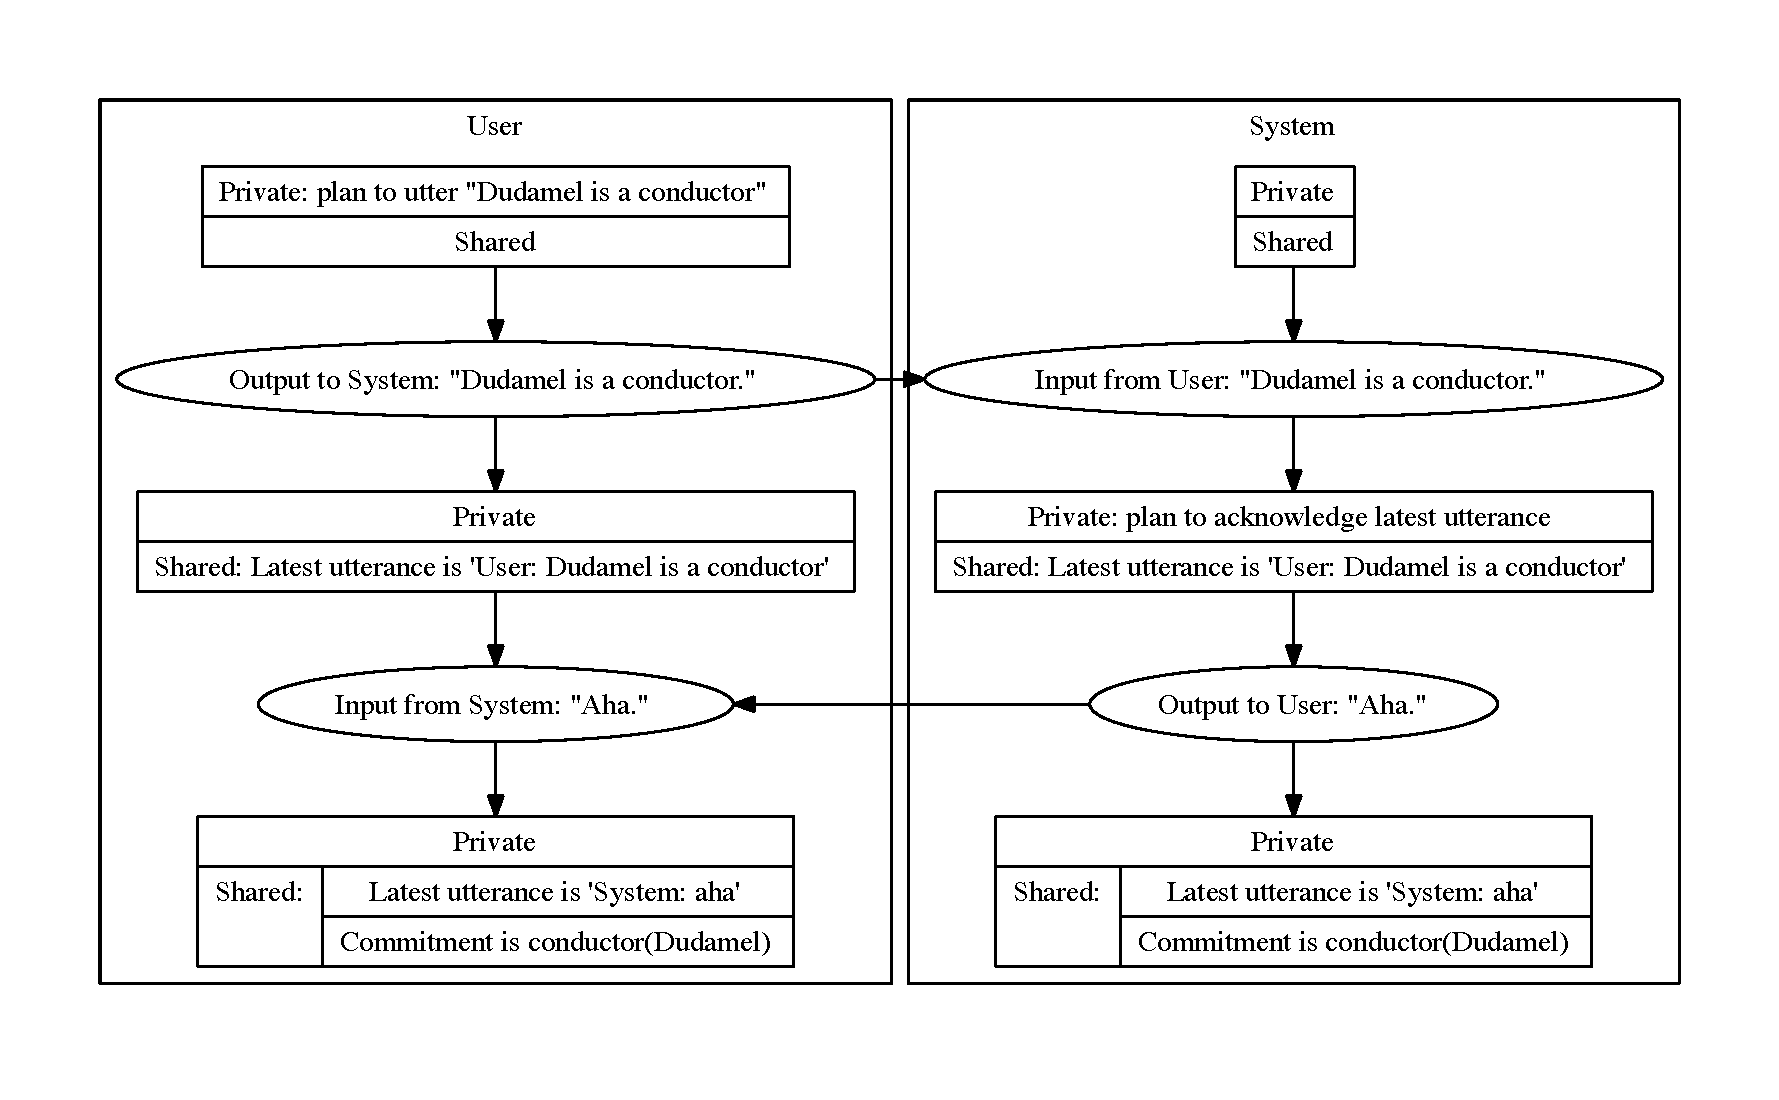
\includegraphics[width=\textheight]{simple-dm-diac}
\caption{Dialogue management:``Dudamel is a conductor''}
\label{fig:simple-dm-diac}
\end{sidewaysfigure}

%\clearpage

This assumes ideal
communication.  There is lots that could go wrong which could have the
consequence that the two agents become misaligned and an important
part of this framework is to provide a basis for the description of
miscommunication as well as communication.  (See
\cite{Ginzburg2012} for more discussion of this.)


We treat the dialogue information states represented by the square
boxes as records as in \nexteg{}.  


\begin{ex} 
\record{\field{private}{\record{\field{agenda}{\textit{AGENDA}}}} \\
        \field{shared}{\record{\field{latest-utterance}{\textit{L-UTT}} \\
                               \field{commitments}{\textit{COMM}}}}} 
\end{ex} 
  

What kinds of objects should \textit{AGENDA}, \textit{L-UTT} and
\textit{COMM} be?  They will be defined with respect to the agent who
owns the information state which, for convenience, we will refer to as
\textit{SELF}.  We will see as we proceed with the discussion below
that \textit{SELF} is related to the notion of \textit{de se} type act discussed in Chapter~\ref{sec:typeacts}.

We will say that \textit{AGENDA} is a list of dialogue move types,
that is,  the types of dialogue moves that \textit{SELF} plans to
realize by means of a creation type act.  Recall from
Chapter~\ref{ch:percint} that this does not necessarily mean that
\textit{SELF} is the main actor in the event realizing the move type.
It can for example be a type of move to be carried out by an
interlocutor which \textit{SELF} should wait for.  This will give us a
mechanism for handling basic turn-taking in dialogue.  (See
\citealp{SacksSchegloffJefferson1974} for the classic work on
turn-taking.) We will define a dependent type \textit{Move} such that for any agent
$A$, \textit{Move}($A$) is the type of dialogue moves in which $A$ is involved.
For now we will say that there are two ways in which an agent can be
involved in a dialogue act:  as speaker (or performer) or as hearer
(part of the audience to whom the dialogue act is
addressed).\footnote{A third way of being involved in a dialogue act
  which we will not take account of here is as an overhearer.}  Performing a dialogue move is a \textit{de se} type act of creation as
discussed in Chapter~\ref{sec:typeacts}.  Being the hearer or audience
of a move type involves a \textit{de se} type act of judgement as
discussed there.
\textit{AGENDA}  should thus be a list of move types depending on
\textit{SELF} (that
is, subtypes of \textit{Move}(\textit{SELF})).  We introduce a
dependent type,
\textit{MoveType}, such that for any $a$:\textit{Ind},
$T$:\textit{MoveType}($a$) iff $T\sqsubseteq\textit{Move}(a)$.
\textit{AGENDA} is thus a list of move types and will
have type [\textit{MoveType}(\textit{SELF})].   For any type $T$, $[T]$ is the type of
lists all of whose members are of type $T$ (see
Appendix~\ref{app:listtypes}).  We will come back to the details of
\textit{Move} below.

\textit{L-UTT} should tell us what move (or moves\footnote{See
  \cite{Larsson2002} for a proposal where dialogue contributions
  involve several moves. For now we will make the simplifying
  assumption that utterances are associated with a single move.}) has just been carried out.
But we will need more information than this.  We will need information about
what (the agent \textit{SELF} thinks) was actually said.  For this we will use a
chart, i.e. a set of edges between vertices representing hypotheses
about parts of the utterance, that is, sign types associated with
parts of the utterance.  The move should be predictable from the chart
by a process of move-interpretation for which we will use the
predicate `m-interp'.  Thus \textit{L-UTT} should itself be of
the type \nexteg{}.

\begin{ex} 
\record{\tfield{move}{\textit{Move}(\textit{SELF})} \\
        \tfield{chart}{\textit{Chart}} \\
        \tfield{e}{m-interp(chart,move)}} 
\end{ex} 
  

The type \textit{Chart}
we will say more about in Chapter~\ref{ch:gram}.

The commitments field has normally been considered as a set of
facts or propositions \citep{Ginzburg2012,Larsson2002}.  Here we will
treat them as a single record type, i.e. a member of the type
\textit{RecType}.  Using a single type will make it more
straightforward to deal with issues like consistency and anaphora [????].

Thus information states can belong to the type \nexteg{}.

\begin{ex} 
\smallrecord{\smalltfield{private}{\smallrecord{\smalltfield{agenda}{[\textit{MoveType}(\textit{SELF})]}}} \\
        \smalltfield{shared}{\smallrecord{\smalltfield{latest-utterance}{\smallrecord{\smalltfield{move}{\textit{Move}(\textit{SELF})} \\
                                                                  \smalltfield{chart}{\textit{Chart}}
                                                                \\
                                                                  \smalltfield{e}{m-interp(chart,move)}}}\\
                               \smalltfield{commitments}{\textit{RecType}}}}} 
\label{ex:InfoStatePrelim}
\end{ex} 
(Here, by convention the labels `chart' and `move' in
\smallrecord{\smalltfield{e}{m-interp(chart,move)}} refer to the path down to the minimal record in
which the e-field occurs, that is `shared.latest-utterance.chart' and
`shared.latest-utterance.move' respectively.)

\preveg{} is, however, not quite general enough.  It requires that
there always will be a latest utterance.  At the beginning of a
dialogue this will not be the case and we need a way of representing
that there is no previous utterance.  We will use a type whose only
witness is the empty record for this.  Records, it will be recalled,
are sets of ordered pairs (see
Appendix~\ref{app:rectypes}).  This will include the empty set,
$\emptyset$ which could also be notated as `[\ ]' if we are thinking
of the empty set as the empty record.  However, this latter notation
is confusing since it could also be used to represent the empty record
type, that is the type that does not place any constraints on which
records it has as witnesses, that is, the type of all records which we
represent as \textit{Rec} in order to avoid confusion.  The type of
the empty record could be constructed as the singleton type
\textit{Rec}$_\emptyset$ (or if you are using the bracket notation for
the empty record, \textit{Rec}$_{[\ ]}$).  In order to avoid
notational confusion we will use \textit{ERec} to represent the type
whose only witness is the empty record, that is, the empty set.  Thus
\nexteg{} will hold.
\begin{ex} 
$a$ : \textit{ERec} iff $a=\emptyset$ 
\end{ex} 
At the beginning of a
dialogue there will not be any shared commitments either.  Therefore, it
will be natural to use \textit{Rec} for the
commitments at the beginning of a dialogue.  \textit{Rec} is the type
of all records.  If we think of records as modelling situations then a
commitment represented by
\textit{Rec} is a commitment to the existence of a situation but not
to a situation of any particular type.  Thus it corresponds to ``there
is a situation'' or ``the world is not empty''.  It plays a similar
role in our theory to the set of all possible worlds in a system based
on possible worlds.  It represents a state where no constraints have
been placed on the nature of the world.   The 
adjustment we need to make to (\ref{ex:InfoStatePrelim}) in order to include dialogue
initial information states is to the shared.latest-utterance field as
in \nexteg{}.  The `commitments'-field does not need to be adjusted as
the type \textit{Rec} is one of the witnesses of \textit{RecType} (see Appendix~\ref{app:rectypes}).
\begin{ex}
\smallrecord{\smalltfield{private}{\smallrecord{\smalltfield{agenda}{[\textit{MoveType}(\textit{SELF})]}}} \\
        \smalltfield{shared}{\smallrecord{\smalltfield{latest-utterance}{\smallrecord{\smalltfield{move}{\textit{Move}(\textit{SELF})} \\
                                                                  \smalltfield{chart}{\textit{Chart}}
                                                                \\
                                                                  \smalltfield{e}{m-interp(chart,move)}}$\vee$\textit{ERec}}\\
                               \smalltfield{commitments}{\textit{RecType}}}}}
\label{ex:gameboard}
\end{ex}
\preveg{} uses a join type (Appendix~\ref{app:jointypes}).  For any two
types $T_1$ and $T_2$ you can form the join (or disjunction) $T_1\vee
T_2$.  $a:T_1\vee T_2$ just in case either $a:T_1$ or $a:T_2$.

\label{pg:SELF}We will use notation including `\textit{SELF}' as in \preveg{} to
represent types which are derived from dependent types by applying
them to the argument represented by \textit{SELF}.  This notational
convention will save us a good deal of complication in presentation
and it is always possible to recover the dependent type from which the
type is derived by creating a function which maps an individual to the
appropriate type.  Thus in the case of \preveg{} the dependent type
would be \nexteg{}.
\begin{ex}
$\lambda a$:\textit{Ind} . \smallrecord{\smalltfield{private}{\smallrecord{\smalltfield{agenda}{[\textit{MoveType}($a$)]}}} \\
        \smalltfield{shared}{\smallrecord{\smalltfield{latest-utterance}{\smallrecord{\smalltfield{move}{\textit{Move}($a$)} \\
                                                                  \smalltfield{chart}{\textit{Chart}}
                                                                \\
                                                                  \smalltfield{e}{m-interp(chart,move)}}$\vee$\textit{ERec}}\\
                               \smalltfield{commitments}{\textit{RecType}}}}}
\end{ex} 
[???? This needs revising in order to include moves by agents other
than \textit{SELF}!]

Dialogue moves are a type of
event in which an actor (normally speaker) is related to an intended
audience, an illocutionary force (such as `assert') and a content
(that is, for our present purposes, a record type such as \smallrecord{\smalltfield{e}{conductor(Dudamel)}}).

% , e.g. assert(User, System,
% conductor(Dudamel)).  We shall need to refine our view of what the
% third argument is.  But for now let us note that assert($a$,$b$,$c$)
% is a \textit{type}.  An object of this type will be an event or
% situation in which $a$ asserts $c$ with $b$ as the intended
% audience. ($b$ may or may not be able hear or comprehend $a$'s
% utterance.)  For technical reasons we will not use this type but one
% where the illocutionary force \textit{assert} is an argument:
% move(User, System, assert, conductor(Dudamel)).  We will need to access the various
% components of move types so that we can partially specify them.
% Therefore we will use the record type

We will take dialogue moves to be a pairing of speech acts and content.
The type of speech acts (\textit{SpeechAct}) will be taken to be a
subtype of the type of speech events (\textit{SEvent}) as defined in
(\ref{ex:SEventLocSpAu}) on p.~\pageref{ex:SEventLocSpAu}.  In
particular this will mean that there is a field in a speech act for
the speaker (labelled by `sp') and another for the audience (labelled
by `au').  More
specifically we will take the type \textit{Move}($a$) to be an abbreviation for
\nexteg{}. 
\begin{ex} 
% \record{\tfield{actor}{\textit{Ind}} \\
%         \tfield{audience}{\{\textit{Ind}\}} \\
%         \tfield{orientation}{eq(\textit{SELF},actor)$\vee$member(\textit{SELF},audience)}
%         \\
%         \tfield{i-force}{\textit{IForce}} \\
%         \tfield{content}{\textit{RecType}} \\
%         \tfield{e}{move(actor, audience, i-force, content)}}
\smallrecord{\smalltfield{e}{\textit{SpeechAct}}} $\wedge$ (
\smallrecord{\smalltfield{e}{\smallrecord{\smallmfield{sp}{$a$}{\textit{Ind}}}}}
$\vee$
\smallrecord{\smalltfield{e}{\smallrecord{\smallmfield{au}{$a$}{\textit{Ind}}}}}
)
$\wedge$ \textit{MoveContent} 
\label{ex:Move-a}
\end{ex}
The type in \preveg{} is a
meet type (Appendix~\ref{app:meettypes}).\footnote{Strictly speaking, this type should be
  written with parentheses since we are assuming a binary meet
  operation:
  (\smallrecord{\smalltfield{e}{\textit{SpeechAct}}} $\wedge$ ((
\smallrecord{\smalltfield{e}{\smallrecord{\smallmfield{sp}{$a$}{\textit{Ind}}}}}
$\vee$
\smallrecord{\smalltfield{e}{\smallrecord{\smallmfield{au}{$a$}{\textit{Ind}}}}}
)
$\wedge$ \textit{MoveContent})) 
  but we will often omit parentheses for clarity.} If $T_1$ and $T_2$ are
types, then an object $a$ is of type  $T_1\wedge T_2$ just in case
$a:T_1$ and $a:T_2$.  

Note that \preveg{} requires $a$ to be either the speaker or the
audience of the speech act and does not rule out the possibility that
$a$ is both speaker and audience (i.e. $a$ is talking to herself).

We
will not attempt a complete inventory of speech act types here.
Preliminarily, we could define \textit{SpeechAct} to be
\begin{quote}
\textit{Assertion}$\vee$\textit{Query}$\vee$\textit{Command}$\vee$\textit{Acknowledgement},
\end{quote}
that
is, a join type (Appendix~\ref{app:jointypes}) of all the available
speech act types.\footnote{Strictly speaking, this type should be
  written with parentheses since we are assuming a binary join
  operation:
  (\textit{Assertion}$\vee$(\textit{Query}$\vee$(\textit{Command}$\vee$\textit{Acknowledgement})))
  but we will often omit parentheses for clarity.}  Something will be of
this type just in case it is of at least one of the types of the
join.  Each of the speech act types are subtypes of \textit{SEvent}
and can be defined as in \nexteg{}.
\begin{ex} 
\begin{tabular}[t]{lcl}
\textit{Assertion} & -- & \textit{SEvent} \d{$\wedge$} 
\smallrecord{\smalltfield{e}{\textit{Phon}} \\
             \smalltfield{c$_{\mathrm{illoc}}$}{assertion(e)}} \\
\textit{Query} & -- & \textit{SEvent} \d{$\wedge$} 
\smallrecord{\smalltfield{e}{\textit{Phon}} \\
             \smalltfield{c$_{\mathrm{illoc}}$}{query(e)}} \\
\textit{Command} & -- & \textit{SEvent} \d{$\wedge$} 
\smallrecord{\smalltfield{e}{\textit{Phon}} \\
             \smalltfield{c$_{\mathrm{illoc}}$}{command(e)}} \\
\textit{Acknowledgement} & -- & \textit{SEvent} \d{$\wedge$} 
\smallrecord{\smalltfield{e}{\textit{Phon}} \\
             \smalltfield{c$_{\mathrm{illoc}}$}{acknowledgement(e)}} 

\end{tabular} 
\end{ex} 
Here the subscript `illoc' stands for ``illocutionary'' indicating
that the condition provides information about the illocutionary force
of the speech act. The symbol \d{$\wedge$} represents the merge operation defined in
Appendix~\ref{app:merge}.  In \preveg{} the relevant merges will be
the unions of the sets of fields represented by \textit{SEvent} and
the type consisting of the `e' and `illoc' fields.  This is
illustrated in \nexteg{} for \textit{Assertion}. \nexteg{a} (where
\textit{SEvent} is spelled out) is
identical with \nexteg{b}.
\begin{ex} 
\begin{subex} 
 
\item \record{\tfield{e-loc}{\textit{Loc}} \\
        \tfield{sp}{\textit{Ind}} \\
        \tfield{au}{\textit{Ind}} \\
        \tfield{e}{\textit{Phon}} \\
        \tfield{c$_{\mathrm{loc}}$}{loc(e,e-loc)} \\
        \tfield{c$_{\mathrm{sp}}$}{speaker(e,sp)} \\
        \tfield{c$_{\mathrm{au}}$}{audience(e,au)}} \d{$\wedge$} 
\smallrecord{\smalltfield{e}{\textit{Phon}} \\
             \smalltfield{c$_{\mathrm{illoc}}$}{assertion(e)}}
 
\item \record{\tfield{e-loc}{\textit{Loc}} \\
        \tfield{sp}{\textit{Ind}} \\
        \tfield{au}{\textit{Ind}} \\
        \tfield{e}{\textit{Phon}} \\
        \tfield{c$_{\mathrm{loc}}$}{loc(e,e-loc)} \\
        \tfield{c$_{\mathrm{sp}}$}{speaker(e,sp)} \\
        \tfield{c$_{\mathrm{au}}$}{audience(e,au)} \\
        \tfield{c$_{\mathrm{illoc}}$}{assertion(e)}}

 
\end{subex} 
   
\end{ex} 
  

Finally, the type \textit{MoveContent} in (\ref{ex:Move-a}) relates the type
of the content of the move to the type of the move.  We define it
preliminarily as the join type in \nexteg{}.
\begin{ex} 
\record{\tfield{e}{\textit{Assertion}} \\
        \tfield{cnt}{\textit{RecType}} \\
        \tfield{c$_{\mathrm{cnt}}$}{content(e,cnt)}}$\vee$
\record{\tfield{e}{\textit{Query}} \\
        \tfield{cnt}{\textit{Question}} \\
        \tfield{c$_{\mathrm{cnt}}$}{content(e,cnt)}}$\vee$
\record{\tfield{e}{\textit{Command}} \\
        \tfield{cnt}{\textit{RecType}} \\
        \tfield{c$_{\mathrm{cnt}}$}{content(e,cnt)}}$\vee$
\record{\tfield{e}{\textit{Acknowledgement}}} 
\end{ex} 
Note that this allows for acknowledgements such as \textit{ok} not to
have any content (although it does not prevent them from having content).  We will return later to discussion of whether this
is a reasonable claim for acknolwedgements, while noting that this would  be one way of
dealing with ``phatic'' communication such as greetings like \textit{Hello}.

% We place a condition on `self' that it be the ``ego'', that is, that
% it involves a situation which is of the type ego(self).  The idea is
% that this is a type \textit{de se} by which we mean that a judgement
% that a situation $s$ is of the type ego($a$) requires that $a$ is the
% individual making the judgement.  We do not have a formal treatment of
% this.  We have relativized our judgements in Appendix~\ref{app:ttr} to
% systems of types involving assignments to the basic types but not to
% the agent making the judgement.  We will not develop this further here
% but merely note that the perception of oneself as the actor or the
% audience of a dialogue move is an essentially \textit{de se}
% phenomenon. For recent discussion of and a survey of the literature on
% \textit{de se} phenomena see \cite{Ninan2010,Hanks2012}.
  

We will be able to read partial information about
a dialogue move from certain aspects of a speech-event.  For example,
an utterance of \textit{ok}
may tell us that the dialogue move is of type \nexteg{}.

\begin{ex} 
% \record{\tfield{actor}{\textit{Ind}} \\
%         \tfield{audience}{\{\textit{Ind}\}} \\
%         \tfield{orientation}{member(\textit{SELF},audience)} \\
%         \mfield{i-force}{acknowledge}{\textit{IForce}} \\
%         \tfield{content}{\textit{RecType}} \\
%         \tfield{e}{move(actor, audience, i-force, content)}} 
\record{\tfield{e}{\textit{Acknowledgement}} \\
        \mfield{sp}{\textit{SELF}}{\textit{Ind}}}
\end{ex} 
If an utterance of \textit{ok} is to have content after all, we will have to look to the previous utterance to find
it.  An
utterance of \textit{Dudamel is a conductor} may give us information
about the type of speech act (\textit{Assertion}) and the content
(\smallrecord{\smalltfield{e}{conductor(Dudamel)}}).  Note, however,
that we only get such a fully specified content if we have a unique
individual `Dudamel' whom we associate with utterances of the name
\textit{Dudamel}.  If the resources we have available do not give us
such an individual associated with \textit{Dudamel} then we only get
the information that somebody named Dudamel is a conductor, that is,
we may only get partial information about the content the speaker
intended to communicate.  Consider the example \textit{Strauss is a
  composer}.  There are at least two famous composers named Strauss
(and also some more not so famous ones).  If our available resources
give us two people associated with the name \textit{Strauss} we will
not know which of them is being referred to.  Representing contents as record types will 
enable us to handle this content underspecification. However, in order
to do this we will need to abandon our current simplifying
``propositional logic'' assumption
that sentences come as unanalyzed wholes associated with their
contents.  This we will do in Chapter~\ref{ch:gram}.
% We will talk
% about the exact nature of the record type when we talk about semantics below.


Not surprisingly, when we are dealing with an agenda as in (\ref{ex:gameboard}), a
plan for future action, we have got ourselves into a situation
where we need types rather than the objects.  The things that are on
the agenda list are not actual events, but rather \textit{types} of
events planned for the future.  Normally the types occurring on the
agenda will be subtypes of \textit{Move}(\textit{SELF}), though we may wish to
include types of events like looking something up in a database,
i.e. non-speech events.

For the most part types on the agenda will not be completely specified
types.  That is they will not be types all of whose fields are
manifest (restricted to particular objects of those types).
Frequently it will be the case that we specify the content of the move
but leave open the phonology, that is, the type will specify the
content of what is to be said but not actually what is to be said or
even perhaps which language it should.  We want, for example, to be able to
say that a speaker is carrying out the same type of move independently of which
language they are speaking.  Thus, if the user says to the system ``Dudamel is a conductor''
or (in Swedish) ``Dudamel �r dirigent'' she will in both cases have carried out a
move involving the assertion of the content \smallrecord{\smalltfield{e}{conductor(Dudamel)}}.  This abstraction will
be important, for example, if we want to change language in the middle
of a dialogue, as people sometimes do.\footnote{This phenomenon is
  known as code-switching \citep{BullockToribio2009}.}  At the same time it is the
normal case to continue a dialogue in the same language and thus we
need to note which language was used in the previous utterance,
i.e. keep track of what was actually said.  This information will be
in the chart which is part of the latest move.  In the chart there
will be
more information about what was actually said which will be important when it comes to dealing
with parts of the utterance for things like clarification and
anaphora.  But this again requires us to abandon our current
simplifying ``propositional logic'' assumption.
    

We will assume that agents do not have complete
information about the information state, that is, they reason in terms
of \textit{types} of information state (that is, gameboards).
The basic intuition behind our reasoning about information state
updates can be expressed as in \nexteg{}.

\begin{ex} 
If $r_i$ : $T_i$, then $r_{i+1}$ : $T_{i+1}(r_i)$ 
\end{ex} 
  

That is, given that we believe that the current information state is
of type $T_i$ (recall that we can come to this belief without having
any belief about which specific information state is involved), then
we can conclude that the next information state is of type $T_{i+1}$
which can depend on the current information state.  According to this,
we can have a hypothesis about the type of the next information state
even though we may not know exactly what the current information state
is.  Exactly which type the next information state belongs to depends,
though, on the exact nature of the current information state.  Thus
the dependency in our types provides us with an additional means for
representing underspecification.

This basic rule of inference corresponds to a function from records to
record types, a function of type ($T_i$ $\rightarrow$ {\it
  RecType\/}), that is, one kind of update function we were using in Chapter~\ref{ch:percint}.  Such a function is of
the form \nexteg{}. 

\begin{ex} 
$\lambda r\!:\!T_i\ .\ T_{i+1}(r)$ 
\end{ex} 
  

Things are a litte more complicated than this, however, because this
only represents the change from one information state to another,
whereas in fact this change is triggered by a speech
event which bears an appropriate relation to the current information
state represented by $r$.  Thus we are actually interested in
functions from the current information state to a function from events
to the new information state, as in \nexteg{}.

\begin{ex}
$\lambda r\!:\!T_i\ .\ \lambda e\!:\!T_e(r)\ .\ T_{i+1}(r,e)$
\label{eg:updateFun}
\end{ex}

This is the other kind of update function we were using in Chapter~\ref{ch:percint}.\footnote{This is
  one of a number of ways of characterizing update in this kind of
  framework.  One might for instance think of the type of the speech event as
  being part of the current information state.  Also instead of using
  an update function one can use a record type with a
  `preconditions'-field and an `effect'-field.  Both
  \cite{Ginzburg2012} and \cite{Larsson2002} have this kind of approach.}  Let us consider
the update function which the user could use in order to update her
information state after her own utterance of \textit{Dudamel is
  a conductor}.  This is modelled on the kind of integration rules
discussed in \cite{Larsson2002}.



\begin{ex} \mbox{}

\hspace*{-3em}\begin{minipage}{\textwidth}$\lambda
r$:\record{\tfield{private}{\record{\tfield{agenda}{$_{\mathit{ne}}$[\textit{MoveType}(\textit{SELF})]}}}}
\\
\hspace*{2em}$\lambda
u$:\record{\tfield{move}{fst($r$.private.agenda)
\d{$\wedge$}
\smallrecord{\smalltfield{e}{\smallrecord{\smallmfield{sp}{\textit{SELF}}{\textit{Ind}}
      \\
                                          \smalltfield{au}{\textit{Ind}}}}}
\d{$\wedge$}
\smallrecord{\smalltfield{e}{\textit{Assertion}}}} \\
                                \tfield{chart}{\textit{Chart}} \\
                                \tfield{e}{m-interp(chart,move)}}\hspace*{.5em}. \\
\hspace*{4em}\smallrecord{\smalltfield{private}{\smallrecord{\smallmfield{agenda}{\begin{tabular}{l}
\smallrecord{\smalltfield{e}{\textit{Acknowledgement}\d{$\wedge$}\smallrecord{\smallmfield{sp}{$u$.move.e.au}{\textit{Ind}}
      \\
                                                                           \smallmfield{au}{\textit{SELF}}{\textit{Ind}}}}
                                                                       \\
             \smallmfield{cnt}{$u$.move.cnt}{\textit{RecType}} \\
             \smalltfield{c$_{\mathrm{cnt}}$}{content(e,cnt)}}  \\
\hspace*{10em}$\mid$ rst($r$.private.agenda) \end{tabular}}{[\textit{MoveType}(\textit{SELF})]}}}
  \\
                      \smalltfield{shared}{\smallrecord{\smalltfield{latest-utterance}{\smallrecord{\smallmfield{move}{$u$.move}{\textit{Move}(\textit{SELF})} \\
                                                                                \smallmfield{chart}{$u$.chart}{\textit{Chart}}
                                                                              \\
\smallmfield{e}{$u$.e}{m-interp(chart,move)}}}}}}
\end{minipage}
\label{eg:updateFunIntegOwn}

\end{ex}



This function maps information states (records), $r$, which have a non-empty
agenda to a function that maps events to a type of information
state. (See Appendix~\ref{app:listtypes} for an account of non-empty
list types.)  It thus requires that the current information state (the
first argument to the function) have a non-empty agenda.  The second
argument to the function (represented by $u$) requires the move
associated with the speech-event to be of the first type on the agenda
in $r$, the current information state, and also to be an assertion
with \textit{SELF} as the speaker (see Appendix~\ref{app:meettypes} for a
discussion of meet types, that is, conjunction).  It also requires that the chart associated
with this utterance can be interpreted as a move of that type.  The
requirements on the arguments to the function represent the
preconditions.  The type that results from applying the function to
its arguments represents the effect of the update.
This type requires the agenda to be result of replacing the first type
on the agenda in $r$ with an acknowledgement where the speaker is the
audience of the assertion move and the audience of the acknolwedgement
is \textit{SELF}.  The content of the acknowledgement is the same as
the content of the assertion.  That is, what is being acknowledged is
the content of the assertion.  It furthermore requires the latest-utterance field to contain the move and chart
of the utterance $u$.  The idea is that
this function should be used to predict the type of the next
information state on the basis of the current information state and
the observed event.  That
is, if we believe the current information state to be of the domain
type of the update function and we observe an event of the required
type then we reason that the updated
information state should be of the type resulting from applying the
function to the current information state.  Thus this update function
will be used in the same way as the update functions we discussed in
Chapter~\ref{ch:percint}.  However, the gameboards involved are now
more complex.



We will now examine how such an update function could be used to
reason about an update.  Let us suppose that the user considers the current information state
to be of type:

\begin{ex}
\smallrecord{\smalltfield{private}{\smallrecord{\smallmfield{agenda}{[
                   \smallrecord{\smalltfield{e}{\textit{Assertion}
                     \d{$\wedge$} \smallrecord{\smallmfield{sp}{\textit{SELF}}{\textit{Ind}}}}                               \\
                                \smallmfield{cnt}{\smallrecord{\smalltfield{e}{conductor(dudamel)}}}{\textit{RecType}}
                                \\
                                \smalltfield{c$_{\mathrm{cnt}}$}{content(e,cnt)}}
]
}{[\textit{RecType}]}}} \\
        \smalltfield{shared}{\smallrecord{\smalltfield{latest-utterance}{\textit{ERec}}\\
                               \smallmfield{commitments}{\textit{Rec}}{\textit{RecType}}}}}
\label{eg:initialInfoDiac}
\end{ex}

This represents that the user intends to assert that Dudamel is a conductor
represented by the record type
\smallrecord{\smalltfield{e}{conductor(Dudamel)}}.  
The user also believes that there was no previous utterance and no commitments,
i.e. that the planned utterance will be dialogue initial.  
% Given the
% assumption that information states may not contain any additional fields, there is no question about what
% the current information state is.  It must be:

% \record{\field{private}{\record{\field{agenda}{$\left[\mbox{\smallrecord{\smallmfield{actor}{User}{\textit{Ind}} \\
%                                                               \smallmfield{audience}{System}{\{\textit{Ind}\}} \\
%                                                               \smallmfield{i-force}{assert}{\textit{IForce}} \\
%                                                               \smallmfield{content}{\smallrecord{\smalltfield{c}{conductor(Dudamel)}}}{\textit{RecType}} \\
%                                                               \smalltfield{c}{move(actor, audience, i-force, content)}}}\right]$}}} \\
%         \field{shared}{\record{\field{latest-utterance}{\record{\field{moves}{$\emptyset$} \\
%                                                                 \field{chart}{$\emptyset$}}}\\
%                                \field{commitments}{[]}}}}

Suppose now that the user utters \textit{Dudamel is a conductor} and
judges this utterance event $u_1$ to be an event of type \nexteg{}.
\begin{ex} 
 \record{\tfield{move}{\smallrecord{\smalltfield{e}{\textit{Assertion}\d{$\wedge$} \smallrecord{\smallmfield{sp}{\textit{SELF}}{\textit{Ind}}}} 
                                \\
                                \smallmfield{cnt}{\smallrecord{\smalltfield{e}{conductor(Dudamel)}}}{\textit{RecType}}
                                \\
                                \smalltfield{c$_{\mathrm{cnt}}$}{content(e,cnt)}}} \\
          \tfield{chart}{\textit{Chart}} \\
          \tfield{e}{m-interp(chart,move)}}
\end{ex} 
  



% \record{\field{moves}{\{$m$\}} \\
%         \field{m}{$m$} \\
%         \field{chart}{$K$}}

% where $m$:\smallrecord{\smallmfield{actor}{User}{\textit{Ind}} \\
%                        \smallmfield{audience}{System}{\{\textit{Ind}\}} \\
%                        \smallmfield{i-force}{assert}{\textit{IForce}} \\
%                        \smallmfield{content}{\smallrecord{\smalltfield{c}{conductor(Dudamel)}}}{\textit{RecType}} \\
%                        \smalltfield{c}{move(actor, audience, i-force,
%                          content)}}
The user will have more information about the nature of the chart
(that is, about what was actually said and how it might be analyzed) than
we have represented but we will leave this underspecified for now.

Clearly in the user's judgement the utterance $u_1$ fulfils the requirements
placed on it by (\ref{eg:updateFunIntegOwn}) since the move
interpretation associated with it is of the type which occurs at
the head of the agenda.  Note that we are reasoning with this function without actually
providing it with an argument since we only have a (hypothesized) type
of the current information state, not the actual information state.
The crucial judgement is that the type of the current information state is
a subtype of the domain type of the function.  This is sufficient to
allow us to come to a conclusion about the type of the new information
state.  

According to the update function the next information state
must be of the type \nexteg{}.

\begin{ex} 
\smallrecord{\smalltfield{private}{\smallrecord{\smallmfield{agenda}{[\smallrecord{\smalltfield{e}{\textit{Acknowledgement}\d{$\wedge$}\smallrecord{\smallmfield{sp}{$u_1$.move.e.au}{\textit{Ind}}
      \\
                                                                           \smallmfield{au}{\textit{SELF}}{\textit{Ind}}}}
                                                                       \\
             \smallmfield{cnt}{$u_1$.move.cnt}{\textit{RecType}} \\
             \smalltfield{c$_{\mathrm{cnt}}$}{content(e,cnt)}}]}{[\textit{RecType}]}}}
  \\
                      \smalltfield{shared}{\smallrecord{\smalltfield{latest-utterance}{\smallrecord{\smallmfield{move}{$u_1$.move}{\textit{Move}} \\
                                                                                \smallmfield{chart}{$u_1$.chart}{\textit{Chart}}
                                                                              \\
\smallmfield{e}{$u_1$.e}{m-interp(chart,move)}}}}}}\label{eg:typepr} 
\end{ex} 
  

% \record{\tfield{private}{\record{\mfield{agenda}{[]}{[\textit{Move}]}}}
%   \\
%                       \tfield{shared}{\record{\tfield{latest-utterance}{\record{\mfield{moves}{\{$m$\}}{\{\textit{Move}\}} \\
%                                                                                 \mfield{chart}{$K$}{\textit{Chart}}}}}}}

\ignore{
Note that we could have come to this conclusion even without the
simplifying assumption that information states cannot contain
additional fields.  Even if the type had been less specified we could
still have drawn the conclusion as long as the agenda field was
specified, e.g. the user might have been unsure whether the dialogue
was already started or not:

\record{\tfield{private}{\record{\mfield{agenda}{[move(User, System, assert, conductor(Dudamel))]}{[\textit{Move}]}}} \\
        \tfield{shared}{\record{\tfield{latest-utterance}{\record{\tfield{moves}{\{\textit{Move}\}} \\
                                                                  \tfield{utterance}{\textit{Chart}}}}\\
                               \tfield{commitments}{\textit{RecType}}}}}
}
But we know more about the new information state than what is
expressed by the type which results from the update function.
Everything we know about the current information state which remains unchanged by the function must be carried
over from the current information state.  This is related to the frame
problem introduced by \cite{McCarthyHayes1969}.\footnote{For a recent
  overview of the frame problem see \cite{Shanahan2009}.}  We 
handle this performing an \textit{asymmetric merge} (see
Appendix~\ref{app:merge}) of the type we have for the current
information state with the type
resulting from the update function.  The asymmetric merge of two types
$T_1$ and $T_2$ is represented by $T_1$\fbox{\d{$\wedge$}}$T_2$.  If
one or both of $T_1$ and $T_2$ are 
non-record types then $T_1$\fbox{\d{$\wedge$}}$T_2$ will be $T_2$. If
they are both record types, then for any label $\ell$ which occurs in
both $T_1$ and $T_2$, $T_1$\fbox{\d{$\wedge$}}$T_2$ will contain a
field labelled $\ell$ with the type resulting from the asymmetric
merge of the corresponding types in the $\ell$-fields of the two types
(in order).  For labels which do not occur in both types,
$T_1$\fbox{\d{$\wedge$}}$T_2$ will contain the fields from $T_1$ and
$T_2$ unchanged.  In this informal statement we have ignored
complications that arise concerning dependent types in record types.
This is discussed in Appendix~\ref{app:merge}.  Our notion of
asymmetric merge is related to the notion of priority unification \citep{Shieber1986}.

Let us see how this works with our example.  We have assumed that the
type under consideration for the
current information state, $T_{\mathit{curr}}$, is
(\ref{eg:initialInfoDiac}) and computed that the predicted type of the updated information
state, $T_{\mathit{pr}}$, is (\ref{eg:typepr}).  Therefore we need to
compute $T_{\mathit{curr}}$\fbox{\d{$\wedge$}}$T_{\mathit{pr}}$, that
is, \nexteg{}.
\begin{ex} 
\smallrecord{\smalltfield{private}{\smallrecord{\smallmfield{agenda}{[\smallrecord{\smalltfield{e}{\textit{Assertion}\d{$\wedge$} \smallrecord{\smallmfield{sp}{\textit{SELF}}{\textit{Ind}}}} 
                                \\
                                \smallmfield{cnt}{\smallrecord{\smalltfield{e}{conductor(Dudamel)}}}{\textit{RecType}}
                                \\
                                \smalltfield{c$_{\mathrm{cnt}}$}{content(e,cnt)}}]}{[\textit{Move}(SELF)]}}} \\
        \smalltfield{shared}{\smallrecord{\smalltfield{latest-utterance}{\textit{ERec}}\\
                               \smallmfield{commitments}{\textit{Rec}}{\textit{RecType}}}}}
\fbox{\d{$\wedge$}}
\smallrecord{\smalltfield{private}{\smallrecord{\smallmfield{agenda}{[\smallrecord{\smalltfield{e}{\textit{Acknowledgement}\d{$\wedge$}\smallrecord{\smallmfield{sp}{$u_1$.move.e.au}{\textit{Ind}}
      \\
                                                                           \smallmfield{au}{\textit{SELF}}{\textit{Ind}}}}
                                                                       \\
             \smallmfield{cnt}{$u_1$.move.cnt}{\textit{RecType}} \\
             \smalltfield{c$_{\mathrm{cnt}}$}{content(e,cnt)}}]}{[\textit{RecType}]}}}
  \\
                      \smalltfield{shared}{\smallrecord{\smalltfield{latest-utterance}{\smallrecord{\smallmfield{move}{$u_1$.move}{\textit{Move}} \\
                                                                                \smallmfield{chart}{$u_1$.chart}{\textit{Chart}}
                                                                              \\
\smallmfield{e}{$u_1$.e}{m-interp(chart,move)}}}}}} 
\end{ex} 
A straightforward way to think of the asymmetric merge of two record
types is in terms of the
paths in each of them.  Both $T_{\mathit{curr}}$ and
$T_{\mathit{pr}}$ contain paths `private.agenda'.  The types at the
end of the respective paths, however,  are distinct singleton types.
(Recall that manifest fields
\smallrecord{\smallmfield{$\ell$}{$a$}{$T$}} are a convenient notation
for \smallrecord{\smalltfield{$\ell$}{$T_a$}} where $T_a$ is a
restriction of the type $T$ whose only witness is $a$.)  Therefore we
include the complete path from the second type in the result of the
asymmetric merge.  In the case of the path `shared.latest-utterance'
we have the type of the empty record \textit{ERec} compared with a
record type of non-empty records
in $T_{\mathit{pr}}$ and since these cannot be merged  we choose the
second record type in the
result.  Finally, the path `shared.commitments'
occurs in the first type but not in the second and therefore it occurs
in its form from the first type in the result of the asymmetric
merge.  The result is given in \nexteg{} which represents the type of
the new information state which has been computed as a result of the update.
\begin{ex} 
\smallrecord{\smalltfield{private}{\smallrecord{\smallmfield{agenda}{[\smallrecord{\smalltfield{e}{\textit{Acknowledgement}\d{$\wedge$}\smallrecord{\smallmfield{sp}{$u_1$.move.e.au}{\textit{Ind}}
      \\
                                                                           \smallmfield{au}{\textit{SELF}}{\textit{Ind}}}}
                                                                       \\
             \smallmfield{cnt}{$u_1$.move.cnt}{\textit{RecType}} \\
             \smalltfield{c$_{\mathrm{cnt}}$}{content(e,cnt)}}]}{[\textit{RecType}]}}}
  \\
                      \smalltfield{shared}{\smallrecord{\smalltfield{latest-utterance}{\smallrecord{\smallmfield{move}{$u_1$.move}{\textit{Move}} \\
                                                                                \smallmfield{chart}{$u_1$.chart}{\textit{Chart}}
                                                                              \\
\smallmfield{e}{$u_1$.e}{m-interp(chart,move)}}}
                        \\
\smallmfield{commitments}{\textit{Rec}}{\textit{RecType}}}}} 
\end{ex} 
  
Why has the field `shared.commitments' not been updated after the user
has asserted that Dudamel is a conductor?  This is because the
audience has not yet confirmed that they have understood and accepted
the move.  We assume that our agents are \textit{cautious} and do not
assume that commitments are shared until the dialogue participant(s)
they are addressing have confirmed acceptance.  This interaction is
known as grounding and is discussed (among other places) in
\cite{Traum1994} and \cite{Larsson2002}.



We shall call the update function (\ref{eg:updateFunIntegOwn})
\textbf{IntegrateOwnAssertion} following the style of \cite{Larsson2002} although
this does not correspond exactly to any of Larsson's particular update
rules.  This then can be used to account for the state that the user
is in after asserting that Dudamel is a conductor.  


We now need an
update function that will account for the effect of this utterance on
another dialogue participant.  For this we will define a function
\textbf{IntegrateOtherAssertion} which allows an agent to integrate a
move which it perceives to be an assertion.


\begin{ex} 
$\lambda
r$:\record{\tfield{private}{\record{\tfield{agenda}{[\textit{RecType}]}}}}
\\
\hspace*{1em}$\lambda
u$:\smallrecord{\smalltfield{move}{\smallrecord{\smalltfield{e}{\textit{Assertion}\d{$\wedge$}\smallrecord{\smalltfield{sp}{\textit{Ind}} \\
                           \smallmfield{au}{\textit{SELF}}{\textit{Ind}}}} 
                                \\
                                \smalltfield{cnt}{\textit{RecType}}
                                \\
                                \smalltfield{c$_{\mathrm{cnt}}$}{content(e,cnt)}}}
                            \\
                \smalltfield{chart}{\textit{Chart}} \\
                \smalltfield{e}{m-interp(chart,move)}}\hspace*{.5em}.
\hspace*{3em}\smallrecord{\smalltfield{private}{\smallrecord{\smallmfield{agenda}{\begin{tabular}{l}\smallrecord{\smalltfield{e}{\textit{Acknowledgement}
\d{$\wedge$}\smallrecord{\smallmfield{sp}{\textit{SELF}}{\textit{Ind}} \\
                           \smallmfield{au}{$u$.move.e.sp}{\textit{Ind}}}} 
                                \\
                                \smallmfield{cnt}{$u$.move.cnt}{\textit{RecType}}
                                \\
                                \smalltfield{c$_{\mathrm{cnt}}$}{content(e,cnt)}} \\
\hspace*{12em}$|\ r$.private.agenda\end{tabular}}{[\textit{RecType}]}}}
  \\
                      \smalltfield{shared}{\smallrecord{\smalltfield{latest-utterance}{\smallrecord{\smallmfield{move}{$u$.move}{\textit{Move}} \\
                                                                                \smallmfield{chart}{$u$.chart}{\textit{Chart}}
                                                                              \\
\smallmfield{e}{$u$.e}{m-interp(chart,move)}}
                                                                          }}}} 
\end{ex} 
If an agent uses \preveg{} to update then the new information state
will contain a move type on the agenda which involves acknowledging
the content of the assertion by the other dialogue partner.  This
update function is also cautious in that it does not yet update the
shared commitments since the acknowledgement is only scheduled on the
agenda but has not yet been performed.  

If an agent performs an acknowledge-event (``ok'')
and it can integrate it with the update function
\textbf{IntegrateOwnAcknowledgement} which will finally perform an
update of shared.commitments.  Before we define this update function
we will examine what needs to happen in order to update the
commitments.  

Suppose that in the dialogue so far it has been established that
Dudamel is a conductor and that this is represented by the record type
\nexteg{}.
\begin{ex} 
\record{\tfield{e}{conductor(Dudamel)}} 
\end{ex} 
Suppose further that the latest move has the content that Beethoven is
a composer, namely \nexteg{}.
\begin{ex} 
\record{\tfield{e}{composer(Beethoven)}} 
\end{ex} 
One obvious way to combine them would be to merge them, that is,
\nexteg{a} which is identical with \nexteg{b} which in turn is
identical with \nexteg{c}, given the definition in
Appendix~\ref{app:merge} which requires that the merge of any two
types which are not both record types is identical with the
meet of the two types.
\begin{ex} 
\begin{subex} 
 
\item \record{\tfield{e}{conductor(Dudamel)}} \nolinebreak\d{$\wedge$} \nolinebreak\record{\tfield{e}{composer(Beethoven)}} 
 
\item
  \record{\tfield{e}{conductor(Dudamel) \d{$\wedge$} composer(Beethoven)}} 

\item \record{\tfield{e}{conductor(Dudamel) $\wedge$ composer(Beethoven)}}
 
\end{subex} 
   
\end{ex} 
For the simple storing of information represented by predicates and
names represented  in (\ref{ex:DudamelBeethoven}) this might be
sufficient.  It makes the claim that all the information is collected
into one eventuality.  In more narrative dialogues referring to
separate events which we may wish to be able to refer back to this
would be an inadequate solution, however.  It would be better if we
have a way of keeping the labels `e' separate so that they don't
clash, for example in \nexteg{a} which is identical with \nexteg{b}
\begin{ex} 
\begin{subex} 
 
\item \record{\tfield{e$_1$}{conductor(Dudamel)}} \nolinebreak\d{$\wedge$} \nolinebreak\record{\tfield{e$_2$}{composer(Beethoven)}} 
 
\item \record{\tfield{e$_1$}{conductor(Dudamel)} \\
              \tfield{e$_2$}{composer(Beethoven)}} 
 
\end{subex} 
   
\end{ex} 
The potential problems of label clash become very clear if we consider
the types in \nexteg{a} corresponding to \textit{a boy hugged a dog}
and \textit{a girl stroked a cat}. \nexteg{a} is identical with
\nexteg{b} and has a single individual which is both a girl and a
boy stroking another individual which is both a dog and a cat.
\begin{ex} 
\begin{subex} 
 
\item \record{\tfield{x}{\textit{Ind}} \\
              \tfield{c$_{\mathrm{boy}}$}{boy(x)} \\
              \tfield{y}{\textit{Ind}} \\
              \tfield{c$_{\mathrm{dog}}$}{dog(y)} \\
              \tfield{e}{hug(x,y)}} \d{$\wedge$} 
      \record{\tfield{x}{\textit{Ind}} \\
              \tfield{c$_{\mathrm{girl}}$}{girl(x)} \\
              \tfield{y}{\textit{Ind}} \\
              \tfield{c$_{\mathrm{cat}}$}{cat(y)} \\
              \tfield{e}{stroke(x,y)}}
 
\item \record{\tfield{x}{\textit{Ind}} \\
              \tfield{c$_{\mathrm{boy}}$}{boy(x)} \\
              \tfield{c$_{\mathrm{girl}}$}{girl(x)} \\
              \tfield{y}{\textit{Ind}} \\
              \tfield{c$_{\mathrm{dog}}$}{dog(y)} \\
              \tfield{c$_{\mathrm{cat}}$}{cat(y)} \\
              \tfield{e}{hug(x,y)$\wedge$stroke(x,y)}} 
 
\end{subex} 
   
\end{ex} 
One way to get around this problem is to ensure that whenever you
introduce new types you always use fresh labels that have not been
used before and then use explicit constraints to require identity in
cases where it is required.  However, when we come to examine
compositional semantics in Chapter~\ref{ch:gram} we will see that it
is quite important to refer to particular labels in our rules of
combination.  Instead of introducing unique \textit{labels} we will
use the power of records to introduce unique \textit{paths} when contents
are combined.  We will use the label `prev' (``previous'').  If
$T_{\mathrm{old}}$ is the content so far and $T_{\mathrm{new}}$ is the
content we wish to add then the new combined content will be as in
\nexteg{a}.  Thus adding the content of \textit{a girl stroked a cat}
to that of \textit{a boy hugged a dog} will yield \nexteg{b}.
\begin{ex} 
\begin{subex} 
 
\item \record{\tfield{prev}{$T_{\mathrm{old}}$}} \d{$\wedge$} $T_{\mathrm{new}}$ 
 
\item \record{\tfield{prev}{\record{\tfield{x}{\textit{Ind}} \\
                                    \tfield{c$_{\mathrm{boy}}$}{boy(x)} \\
                                    \tfield{y}{\textit{Ind}} \\
                                    \tfield{c$_{\mathrm{dog}}$}{dog(y)} \\
                                    \tfield{e}{hug(x,y)}}} \\
              \tfield{x}{\textit{Ind}} \\
              \tfield{c$_{\mathrm{girl}}$}{girl(x)} \\
              \tfield{y}{\textit{Ind}} \\
              \tfield{c$_{\mathrm{cat}}$}{cat(y)} \\
              \tfield{e}{stroke(x,y)}} 
 
\end{subex} 
   
\end{ex} 
In the case of our example with Dudamel and Beethoven the result will
be \nexteg{}.
\begin{ex} 
\record{\tfield{prev}{\record{\tfield{e}{conductor(Dudamel)}} \\
        \tfield{e}{composer(Beethoven)}}} 
\end{ex} 
If we add a further fact to this, say, that Uchida is a pianist we
would obtain \nexteg{}
\begin{ex} 
\record{\tfield{prev}{\record{\tfield{prev}{\record{\tfield{e}{conductor(Dudamel)}} \\
                               \tfield{e}{composer(Beethoven)}}}} \\
        \tfield{e}{pianist(Uchida)}} 
\end{ex} 
This means that we now have to add additional information if we want
to require identity, for example if we want the Beethoven and Uchida
eventualities (prev.e and e in \preveg{}) to be identical.  We will
return to these matters when we deal with anaphora in
Chapter~\ref{ch:gram}.  Note that this strategy also gives us a
straightforward record of the order in which content was added.

The update function \textbf{IntegrateOwnAcknowledgement} is given in \nexteg{}.
\begin{ex} 
$\lambda
r$:\record{\tfield{private}{\record{\tfield{agenda}{$_{\mathit{ne}}$[\textit{RecType}]}}}\\
           \tfield{shared}{\record{\tfield{latest-utterance}{
                                      \record{\tfield{move}{
                                            \record{\tfield{content}{\textit{RecType}}}}}}
                                    \\
                                   \tfield{commitments}{\textit{RecType}}}}}
\\
\hspace*{1em}$\lambda
u$:\record{\tfield{move}{fst($r$.private.agenda)\d{$\wedge$}\smallrecord{
\smalltfield{e}{\textit{Acknowledgement}}}\d{$\wedge$}\smallrecord{\smalltfield{e}{\smallrecord{\smallmfield{sp}{\textit{SELF}}{\textit{Ind}}}}}
} \\
           \tfield{chart}{\textit{Chart}} \\
           \tfield{e}{m-interp(chart,move)}}\hspace*{.5em}. \\
\hspace*{2em}\smallrecord{\smalltfield{private}{\smallrecord{\smallmfield{agenda}{rst($r$.private.agenda)}{[\textit{RecType}]}}}
  \\
                      \smalltfield{shared}{\smallrecord{\smalltfield{latest-utterance}{\smallrecord{\smallmfield{move}{$u$.move}{\textit{Move}} \\
                                                                                \smallmfield{chart}{$u$.chart}{\textit{Chart}}
                                                                              \\
\smallmfield{e}{$u$.e}{m-interp(chart,move)}}}
                        \\
\smallmfield{commitments}{\smallrecord{\smalltfield{prev}{$r$.commitments}}\d{$\wedge$}$u$.move.cnt}{\textit{RecType}}}}} 
\end{ex} 
This function will
\begin{enumerate} 
 
\item update the agenda with the result of removing the first item on
  the agenda in $r$, the information state prior to update 
 
\item update the latest utterance with the current utterance (e.g. the
  utterance of \textit{ok})

\item update the commitments to be the result of placing the
  commitments of $r$ under the label `prev'  and merging with the
  content of the move in the acknolwedgement, $u$,
  (which by the update function \textbf{IntegrateOtherAssertion} will
  be the content of the previous assertion, e.g. the utterance of \textit{Dudamel is a conductor}) 
 
\end{enumerate} 
    


We then need an update function
  \textbf{IntegrateOtherAcknowledgement} which 
is like \textbf{IntegrateOwnAcknowledgment} except that it requires
that the move event is directed towards the agent doing the updating.  This is given in \nexteg{}.
\begin{ex} 
$\lambda
r$:\record{\tfield{private}{\record{\tfield{agenda}{$_{\mathit{ne}}$[\textit{RecType}]}}}\\
           \tfield{shared}{\record{\tfield{latest-utterance}{
                                      \record{\tfield{move}{
                                            \record{\tfield{content}{\textit{RecType}}}}}}
                                    \\
                                   \tfield{commitments}{\textit{RecType}}}}}
\\
\hspace*{1em}$\lambda
u$:\record{\tfield{move}{fst($r$.private.agenda)\d{$\wedge$}\smallrecord{
\smalltfield{e}{\textit{Acknowledgement}}}\d{$\wedge$}\smallrecord{\smalltfield{e}{\smallrecord{\smallmfield{au}{\textit{SELF}}{\textit{Ind}}}}}
} \\
           \tfield{chart}{\textit{Chart}} \\
           \tfield{e}{m-interp(chart,move)}}\hspace*{.5em}. \\
\hspace*{2em}\smallrecord{\smalltfield{private}{\smallrecord{\smallmfield{agenda}{rst($r$.private.agenda)}{[\textit{RecType}]}}}
  \\
                      \smalltfield{shared}{\smallrecord{\smalltfield{latest-utterance}{\smallrecord{\smallmfield{move}{$u$.move}{\textit{Move}} \\
                                                                                \smallmfield{chart}{$u$.chart}{\textit{Chart}}
                                                                              \\
\smallmfield{e}{$u$.e}{m-interp(chart,move)}}}
                        \\
\smallmfield{commitments}{\smallrecord{\smalltfield{prev}{$r$.commitments}}\d{$\wedge$}$u$.move.cnt}{\textit{RecType}}}}} 
\end{ex}


% Note that neither of these update functions place constraints on the
% content of the acknowledgement but rather update the commitments with
% the content of the previous utterance.  This leaves the way open for
% giving an analysis of acknowledgements without any propositional
% content.  Their occurrence in a dialogue serves as an instruction to
% add the content of the previous utterance not the current utterance.
% Thus we see how dialogue moves can make a procedural contribution
% (``update the commitments with the content of the previous
% utterance!'') rather than expressing a propositional content
% themselves.


We have so far talked of update functions in this chapter, functions
which given an information state and an utterance will return
a type for an updated information state.  Update functions specify
something about the state that an agent will be in after the
occurrence of a certain type of event.  We have not, however,
specified what it is that will specify that an agent should carry out
an action which gives rise to an event of the appropriate
type. Formally, these will also be functions which map an information
state of a given type to a new type, the type of event which the agent
is to bring about.  Thus they too will be functions from objects to
types (or dependent functions).  We will call such functions
\textit{action functions}.  These are associated with creation type
acts (Chapter~\ref{sec:typeacts}).  We will introduce one such function,
\textbf{ExecTopAgenda}, which takes an information state with a
non-empty agenda and returns a type for a move of that type and a
chart which can be interpreted as that move.  It is given in
\nexteg{}.
\begin{ex} 
$\lambda
r$:\record{\tfield{private}{\record{\tfield{agenda}{$_{\mathit{ne}}$[\textit{RecType}]}}}}\hspace*{.5em}.
\\
\hspace*{2em}\record{\tfield{move}{fst($r$.private.agenda)} \\
                                \tfield{chart}{\textit{Chart}} \\
                                \tfield{e}{m-interp(chart,move)}} 
\label{eg:ExecTopAgenda}
\end{ex} 

\section{Resources}

While there is no formal distinction between update functions and
action functions they are to be used in different ways.  Update
functions are to be used as instructions to conclude that there is
something of the resulting type. Action functions are to be used as
instructions to create something of the resulting type.  We shall say that they are different kinds of
\textit{resources} that are available to an agent. The update and
action functions we have discussed in this chapter belong to a general
resource for \textit{dialogue management}.  We shall see that there
are a number of resources which contain both update and action
functions and that in general they can be viewed as the two kinds of
enthymemes (inferential and imperative) discussed in Breitholtz' work
in progress on Aristotelian enthymemes \citep{BreitholtzVilling2008,Breitholtz2010,BreitholtzCooper2011}.

We need more resources:  signs and move-interpretations of charts
containing signs.  In this chapter we are taking signs to be objects
of type (\ref{eg:infex-sign-type}) and the sign corresponding to
\textit{Dudamel is a conductor} is (\ref{eg:diac}).  For compactness
of representation we can define an operation which takes a speech
event type and a content and constructs the corresponding sign.  This
can be defined as in \nexteg{}.
\begin{ex} 
If $\sigma$ is a type of speech event and $\kappa$ is a type (of
situation) then \\
sign($\sigma$,$\kappa$)= \smallrecord{\smalltfield{s-event}{\smallrecord{\smalltfield{e}{$\sigma$}} } \\
        \mfield{cnt}{\smallrecord{\smalltfield{e}{$\kappa$} \\
                             \smalltfield{c$_{\mathrm{tns}}$}{final\_align($\Uparrow$s-event.e,e)}}}{\textit{RecType}}} 
\end{ex} 
Note that the operation `sign' introduces the interpretation of
present tense (represented by the field `c$_{\mathrm{tns}}$').  This
is only possible because the resources we are considering concern only
simple present tense assertions such as \textit{Dudamel is a
  conductor}.  We will see already in the next chapter that things are
not this simple.  We can use \preveg{} to create signs types for
utterances with specific contents such as \textit{Dudamel is a
  conductor} or \textit{Beethoven is a composer}.  We will use another
operation `sign$_{\mathit{uc}}$' to create signs with underspecified
content as defined in \nexteg{}.
\begin{ex} 
If $\sigma$ is a type of speech event then \\
sign$_{\mathit{uc}}$($\sigma$)= \smallrecord{\smalltfield{s-event}{\smallrecord{\smalltfield{e}{$\sigma$}} } \\
        \smalltfield{cnt}{\textit{RecType}}} 
\end{ex}
Now we can characterize the sign types that an agent that can deal
with the simple dialogues that we have been characterizing in this
chapter as \nexteg{}.
\begin{ex} 
\{sign(``Dudamel is a conductor'', conductor(dudamel)), \\ 
\hspace*{1em}sign(``Beethoven
is a composer'', composer(beethoven)), \\
\hspace*{1em}sign(``Uchida is a
pianist'', pianist(uchida)), \\
\hspace*{1em}sign$_{\mathit{uc}}$(``ok''), \\
\hspace*{1em}sign$_{\mathit{uc}}$(``aha'')\}
\label{eg:signdef}
 
\end{ex} 
Recall that ``Dudamel is a conductor'' etc. represent a type of a
string of word utterance events.  For any word $w$, ``$w$'' is the
type of event where $w$ is uttered.  For present purposes we assume
that  the agent has basic types of word utterances as given in
\nexteg{a}.  In order to cope with the content the agent must have a
basic type \textit{Ind} to which certain individuals belong as given
in \nexteg{b}.  Finally in order to construct the ptypes used for the
content the agent would have to have the predicates given in
\nexteg{c}.
\begin{ex} 
\begin{subex} 
 
\item ``Dudamel'', ``is'', ``a'', ``conductor'', ``Beethoven'',
  ``composer'', ``Uchida'', ``pianist'', ``aha'', ``ok'' 
 
\item dudamel, beethoven, uchida : \textit{Ind}

\item predicates with arity $\langle$\textit{Ind}$\rangle$:  conductor, composer, pianist 
 
\end{subex} 
   
\end{ex} 
The set of ptypes based on \preveg{b,c} is thus \nexteg{}.
\begin{ex} 
\{$p(a)$ $\mid$
$p\in\{\mathrm{conductor},\mathrm{composer},\mathrm{pianist}\}$ and \\
\hspace*{3em}$a\in\{\mathrm{dudamel},\mathrm{beethoven},\mathrm{uchida}\}$\} 
\end{ex} 
Of the ptypes in \preveg{} we could say that `conductor(dudamel)',
`composer(beethoven)' and `pianist(uchida)' are non-empty (``true'')
and the rest are empty, although that may not correspond to the actual
facts of the world.  (Beethoven was a pianist, for example.)  Very
often, we are mainly interested in whether a ptype has witnesses
(something of the type) or not and not particularly what those
witnesses are.  In a complete formal treatment, of course, the type
system would specify objects which belong to those types.  For
example, we could say $s_1$ : conductor(dudamel),
$s_2$ : composer(beethoven) and $s_3$ : pianist(uchida).  Informally, we
can say $s_1$ is a situation where Dudamel is a conductor or which
shows that Dudamel is a conductor and so on.  The idea of saying that
an agent has a certain type in its resources is not so much to say
that it has complete information about what belongs to the type
(although its memory will contain partial information about what
belongs to what types) but
rather that it has a way (possibly not entirely decidable) of recognizing an object of the type if
it sees one.  Thus since I am an agent with the type
`composer(uchida)' in my resources I know (sort of) what it would mean
for a situation to be of this type, e.g. a situation in which Uchida
has written original musical compositions, had them performed and so
on.  When we are using our type theory to give an analysis of certain
fragments of language we are sometimes interested in going into more
detail concerning the criteria for belonging to a given type.  Other
times we just treat the type as basic and only need to assume that the
agent has some way of recognizing objects of the type.  It depends on
the level of detail we are interested in for the particular analysis.

We have used predicates other than those given in \preveg{} in the
types that we have discussed in this chapter.  There are ``technical''
predicates such as `m-interp' (``move interpretation'') which takes as
its arguments a chart and a move.  If $c$ is a chart and $m$ is a move
then m-interp($c$,$m$) will be a non-empty type just in case ``$m$ is
an interpretation of $c$''.  Clearly, this is a case where it is of
theoretical interest to us to say more about what constraints this
places on $c$ and $m$.

For the purposes of this chapter, since the parsing involved is a
trivial association of strings of words with signs without any
constituent analysis, we will equate charts with signs, that is $a$ :
\textit{Chart} just in case $a$ : \textit{Sign}.  Thus `m-interp' will
relate signs to moves.  The definition is given in \nexteg{}.
\begin{ex} 
\begin{subex} 
 
\item if $c$ : \textit{Chart} and $m$ : \textit{Move} and for some $\sigma$ and $\kappa$, $c$=sign($\sigma$,$\kappa$),
  then m-interp($c$,$m$) is non-empty iff $m$ : 
\smallrecord{\smalltfield{e}{\textit{Assertion}} \\
             \smallmfield{cnt}{$c$.cnt}{\textit{RecType}}} 
 
\item if $c$ : \textit{Chart} and $m$ : \textit{Move} and for some
  $\sigma$, $c$=sign$_{uc}$($\sigma$),  then m-interp($c$,$m$) is
  non-empty iff $m$ :
\smallrecord{\smalltfield{e}{\textit{Acknowledgement}} \\
             \smalltfield{cnt}{\textit{RecType}}}
 
\end{subex} 
   
\end{ex}
% The role that SELF plays in the move is determined by whether SELF is
% the speaker or the audience in the speech event as defined in \nexteg{}.
% \begin{ex} 
% if $c$ : \textit{Chart} and $m$ : \textit{Move} and m-interp($c$,$m$)
% is non-empty, then $c$.s-event.sp=SELF implies $m$ :
% \smallrecord{\smalltfield{e}{\textit{SpeechAct}} \\
%              \smalltfield{c$_{\mathrm{SELF}}$}{actor(e,SELF)}} and \\
% $c$.s-event.au=SELF implies $m$ :
% \smallrecord{\smalltfield{e}{\textit{SpeechAct}} \\
%              \smalltfield{c$_{\mathrm{SELF}}$}{addressed(e,SELF)}}
% \end{ex} 

Let us now check that we can characterize the types of information
states of $A$ and $B$ in the dialogue \nexteg{}, where we represent
the information states associated with the two agents at various
points in the dialogue as $a_i$ and $b_i$, and the utterance events as $u_i$.
\begin{ex} 
\begin{tabular}[t]{llc}
\multicolumn{2}{c}{$a_0$,$b_0$} & \\
A: & Dudamel is a conductor & $u_1$ \\
\multicolumn{2}{c}{$a_1$,$b_1$} & \\
B: & Aha & $u_2$\\
\multicolumn{2}{c}{$a_2$,$b_2$} & \\
A: & Beethoven is a composer & $u_3$ \\
\multicolumn{2}{c}{$a_3$,$b_3$} & \\
B: & ok & $u_4$ \\
\multicolumn{2}{c}{$a_4$,$b_4$} & \\
A: & Uchida is a pianist & $u_5$ \\
\multicolumn{2}{c}{$a_5$,$b_5$} & \\
B: & ok & $u_6$ \\
\multicolumn{2}{c}{$a_6$,$b_6$} & 
\end{tabular} 
\label{ex:ass-ack-dial}
\end{ex} 
We will assume that $a_0$ and $b_0$ are initial states, essentially
empty except for $A$'s agenda to make the three assertions.  This is
shown in \nexteg{}.
\begin{ex} 
\begin{subex} 
 
\item $a_0$ : \smallrecord{\smalltfield{private}{\smallrecord{\smallmfield{agenda}{[
                   \smallrecord{\smalltfield{e}{\textit{Assertion} \d{$\wedge$}
\smallrecord{\smallmfield{sp}{\textit{SELF}}{\textit{Ind}}}} 
                                \\
                                \smallmfield{cnt}{\smallrecord{\smalltfield{e}{conductor(dudamel)}}}{\textit{RecType}}
                                \\
                                \smalltfield{c$_{\mathrm{cnt}}$}{content(e,cnt)}}, \\
\hspace*{5em}\smallrecord{\smalltfield{e}{\textit{Assertion} \d{$\wedge$}
\smallrecord{\smallmfield{sp}{\textit{SELF}}{\textit{Ind}}}} 
                                \\
                                \smallmfield{cnt}{\smallrecord{\smalltfield{e}{composer(beethoven)}}}{\textit{RecType}}
                                \\
                                \smalltfield{c$_{\mathrm{cnt}}$}{content(e,cnt)}}, \\
\hspace*{6em}\smallrecord{\smalltfield{e}{\textit{Assertion} \d{$\wedge$}
\smallrecord{\smallmfield{sp}{\textit{SELF}}{\textit{Ind}}}} 
                                \\
                                \smallmfield{cnt}{\smallrecord{\smalltfield{e}{pianist(uchida)}}}{\textit{RecType}}
                                \\
                                \smalltfield{c$_{\mathrm{cnt}}$}{content(e,cnt)}}
]
}{[\textit{RecType}]}}} \\
        \smalltfield{shared}{\smallrecord{\smalltfield{latest-utterance}{\textit{ERec}}\\
                               \smallmfield{commitments}{\textit{Rec}}{\textit{RecType}}}}}  
 
\item $b_0$ :  \smallrecord{\smalltfield{private}{\smallrecord{\smallmfield{agenda}{\textit{Rec}}{[\textit{RecType}]}}} \\
        \smalltfield{shared}{\smallrecord{\smalltfield{latest-utterance}{\textit{ERec}}\\
                               \smallmfield{commitments}{\textit{Rec}}{\textit{RecType}}}}} 
 
\end{subex} 
\label{eg:initial-states}   
\end{ex} 
\preveg{} indicates that $a_0$ is an appropriate argument to the
function \textbf{ExecTopAgenda} given in (\ref{eg:ExecTopAgenda}) and
repeated in Appendix~\ref{app:dialrules}.  The result of applying
\textbf{ExecTopAgenda} to $a_0$ is given in \nexteg{}.
\begin{ex} 
\textbf{ExecTopAgenda}($a_0$) = 
\smallrecord{\smalltfield{move}{\smallrecord{\smalltfield{e}{\textit{Assertion}
     \d{$\wedge$}
\smallrecord{\smallmfield{sp}{\textit{SELF}}{\textit{Ind}}} } 
                                \\
                                \smallmfield{cnt}{\smallrecord{\smalltfield{e}{conductor(dudamel)}}}{\textit{RecType}}
                                \\
                                \smalltfield{c$_{\mathrm{cnt}}$}{content(e,cnt)}}}
                            \\
             \smalltfield{chart}{\textit{Chart}} \\
             \smalltfield{e}{m-interp(chart,move)}} 
\label{eg:exectopag(a0)}
\end{ex} 
Note that given our notational convention on using \textit{SELF} (p.~\pageref{pg:SELF}), \preveg{} is
actually a dependent type as in \nexteg{}.
\begin{ex} 
$\lambda a$:\textit{Ind} . \smallrecord{\smalltfield{move}{\smallrecord{\smalltfield{e}{\textit{Assertion}\d{$\wedge$}
\smallrecord{\smallmfield{sp}{$a$}{\textit{Ind}}}} 
                                \\
                                \smallmfield{cnt}{\smallrecord{\smalltfield{e}{conductor(dudamel)}}}{\textit{RecType}}
                                \\
                                \smalltfield{c$_{\mathrm{cnt}}$}{content(e,cnt)}}}
                            \\
             \smalltfield{chart}{\textit{Chart}} \\
             \smalltfield{e}{m-interp(chart,move)}} 
\end{ex} 
This means that the appropriate licensing condition on type acts
associated with \textbf{ExecTopAgenda} (given in
Appendix~\ref{app:actfuns}) is the \textit{de se} variant in \nexteg{}.
\begin{ex} 
If
$f:(T\rightarrow(\textit{Ind}\rightarrow\textit{Type}))$ is an action function then for any
object $a$ and agent $A$, $a:_A T$ licenses $:_A f(a)(A)!$ 
\end{ex} 
That is, $A$ is licensed to create (or contribute to the creation of) something of the type
(\ref{eg:exectopag(a0)}) with $A$ itself as \textit{SELF}.  We have not yet
said anything about what is involved in creating something of this
type.  The procedure involves generating a chart (in this chapter
conceived of as a sign) whose content corresponds to the content of
the move.  We will not make this formally precise here but will wait
until Chapter~\ref{ch:gram} where we have developed a more serious
approach to grammar.  Suffice it to say that the agent's resources
must include the sign types introduced in
(\ref{eg:signdef}) and that there is just one sign type here involving the
type `conductor(dudamel)' which figures in the content of the move
specified in (\ref{eg:exectopag(a0)}), namely sign(``Dudamel is a
conductor'', conductor(dudamel)).  For convenience we will abbreviate
the notation of this type as \signtype{``Dudamel is a conductor''}.  Only a sign of this type will
satisfy m-interp for a move of the move type.  Thus in order to
realize something of type (\ref{eg:exectopag(a0)}) $A$ must in fact
create something of type \nexteg{}, a subtype of
(\ref{eg:exectopag(a0)}).
\begin{ex} 
\record{\tfield{move}{\record{\tfield{e}{\textit{Assertion} \d{$\wedge$}
\smallrecord{\smallmfield{sp}{\textit{SELF}}{\textit{Ind}}}} 
                                \\
                                \mfield{cnt}{\smallrecord{\smalltfield{e}{conductor(dudamel)}}}{\textit{RecType}}
                                \\
                                \tfield{c$_{\mathrm{cnt}}$}{content(e,cnt)}}}
                            \\
             \tfield{chart}{\signtype{``Dudamel is a conductor''}} \\
             \tfield{e}{m-interp(chart,move)}} 
\end{ex}
(Here it is important that \signtype{``Dudamel is a conductor''} is an
abbreviation for the \textit{notation} of the sign type, since when
the notation is interpreted \textit{in situ} in \preveg{} each
local path-name occurring as an argument to a predicate will be prefixed by
`chart.' and thus what occurs in the `chart'-field of \preveg{} is
actually a modified version of the original type.  It is possible to
develop a notation that is more explicit but it becomes cluttered and unwieldy.)

Thus we can conclude that $u_1$ is judged by $A$ to be of type \preveg{}.  We can now
predict that $a_1$ is of type
\textbf{IntegrateOwnAssertion}($a_0$)($u_1$) which, given the types we
have hypothesized for $a_0$ and $u_1$ will be \nexteg{}.
\begin{ex} 
\smallrecord{\smalltfield{private}{\smallrecord{\smallmfield{agenda}{[
\smallrecord{\smalltfield{e}{\textit{Acknowledgement}\d{$\wedge$}\smallrecord{\smallmfield{sp}{$u_1$.move.e.au}{\textit{Ind}}
      \\
                                                                           \smallmfield{au}{\textit{SELF}}{\textit{Ind}}}}
                                                                       \\
             \smallmfield{cnt}{$u_1$.move.cnt}{\textit{RecType}} \\
             \smalltfield{c$_{\mathrm{cnt}}$}{content(e,cnt)}}, \\
\hspace*{5em}\smallrecord{\smalltfield{e}{\textit{Assertion}
          \d{$\wedge$}
\smallrecord{\smallmfield{sp}{\textit{SELF}}{\textit{Ind}}}} 
                                \\
                                \smallmfield{cnt}{\smallrecord{\smalltfield{e}{composer(beethoven)}}}{\textit{RecType}}
                                \\
                                \smalltfield{c$_{\mathrm{cnt}}$}{content(e,cnt)}}, \\
\hspace*{7em}\smallrecord{\smalltfield{e}{\textit{Assertion} \d{$\wedge$}
\smallrecord{\smallmfield{sp}{\textit{SELF}}{\textit{Ind}}}} 
                                \\
                                \smallmfield{cnt}{\smallrecord{\smalltfield{e}{pianist(uchida)}}}{\textit{RecType}}
                                \\
                                \smalltfield{c$_{\mathrm{cnt}}$}{content(e,cnt)}}
]}{[\textit{RecType}]}}} \\
\smalltfield{shared}{\smallrecord{\smalltfield{latest-utterance}{\smallrecord{\smallmfield{move}{$u_1$.move}{\smallrecord{\smalltfield{e}{\textit{Assertion}
            \d{$\wedge$}
\smallrecord{\smallmfield{sp}{\textit{SELF}}{\textit{Ind}}}} 
                                \\
                                \smallmfield{cnt}{\smallrecord{\smalltfield{e}{conductor(dudamel)}}}{\textit{RecType}}
                                \\
                                \smalltfield{c$_{\mathrm{cnt}}$}{content(e,cnt)}}}\\
\smallmfield{chart}{$u_1$.chart}{\signtype{``Dudamel is a conductor''}} \\
\smallmfield{e}{$u_1$.e}{m-interp(chart,move)}}}}}}
 
\end{ex} 
We can now use \preveg{} to update the type we had for $a_0$, given in
(\ref{eg:initial-states}a), as in \nexteg{a} which is identical with
\nexteg{b}.
\begin{ex} 
\begin{subex} 
 
\item \smallrecord{\smalltfield{private}{\smallrecord{\smallmfield{agenda}{[
                   \smallrecord{\smalltfield{e}{\textit{Assertion} \d{$\wedge$}
\smallrecord{\smallmfield{sp}{\textit{SELF}}{\textit{Ind}}}} 
                                \\
                                \smallmfield{cnt}{\smallrecord{\smalltfield{e}{conductor(dudamel)}}}{\textit{RecType}}
                                \\
                                \smalltfield{c$_{\mathrm{cnt}}$}{content(e,cnt)}}, \\
\hspace*{5em}\smallrecord{\smalltfield{e}{\textit{Assertion} \d{$\wedge$}
\smallrecord{\smallmfield{sp}{\textit{SELF}}{\textit{Ind}}}} 
                                \\
                                \smallmfield{cnt}{\smallrecord{\smalltfield{e}{composer(beethoven)}}}{\textit{RecType}}
                                \\
                                \smalltfield{c$_{\mathrm{cnt}}$}{content(e,cnt)}}, \\
\hspace*{6em}\smallrecord{\smalltfield{e}{\textit{Assertion} \d{$\wedge$}
\smallrecord{\smallmfield{sp}{\textit{SELF}}{\textit{Ind}}}} 
                                \\
                                \smallmfield{cnt}{\smallrecord{\smalltfield{e}{pianist(uchida)}}}{\textit{RecType}}
                                \\
                                \smalltfield{c$_{\mathrm{cnt}}$}{content(e,cnt)}}
]
}{[\textit{RecType}]}}} \\
        \smalltfield{shared}{\smallrecord{\smalltfield{latest-utterance}{\textit{ERec}}\\
                               \smallmfield{commitments}{\textit{Rec}}{\textit{RecType}}}}}  
\fbox{\d{$\wedge$}} \\
\smallrecord{\smalltfield{private}{\smallrecord{\smallmfield{agenda}{[\smallrecord{\smalltfield{e}{\textit{Acknowledgement}\d{$\wedge$}\smallrecord{\smallmfield{sp}{$u_1$.move.e.au}{\textit{Ind}}
      \\
                                                                           \smallmfield{au}{\textit{SELF}}{\textit{Ind}}}}
                                                                       \\
             \smallmfield{cnt}{$u_1$.move.cnt}{\textit{RecType}} \\
             \smalltfield{c$_{\mathrm{cnt}}$}{content(e,cnt)}}, \\
\hspace*{5em}\smallrecord{\smalltfield{e}{\textit{Assertion}
          \d{$\wedge$}
\smallrecord{\smallmfield{sp}{\textit{SELF}}{\textit{Ind}}}} 
                                \\
                                \smallmfield{cnt}{\smallrecord{\smalltfield{e}{composer(beethoven)}}}{\textit{RecType}}
                                \\
                                \smalltfield{c$_{\mathrm{cnt}}$}{content(e,cnt)}}, \\
\hspace*{7em}\smallrecord{\smalltfield{e}{\textit{Assertion} \d{$\wedge$}
\smallrecord{\smallmfield{sp}{\textit{SELF}}{\textit{Ind}}}} 
                                \\
                                \smallmfield{cnt}{\smallrecord{\smalltfield{e}{pianist(uchida)}}}{\textit{RecType}}
                                \\
                                \smalltfield{c$_{\mathrm{cnt}}$}{content(e,cnt)}}
]}{[\textit{RecType}]}}} \\
\smalltfield{shared}{\smallrecord{\smalltfield{latest-utterance}{\smallrecord{\smallmfield{move}{$u_1$.move}{\smallrecord{\smalltfield{e}{\textit{Assertion}
            \d{$\wedge$}
\smallrecord{\smallmfield{sp}{\textit{SELF}}{\textit{Ind}}}} 
                                \\
                                \smallmfield{cnt}{\smallrecord{\smalltfield{e}{conductor(dudamel)}}}{\textit{RecType}}
                                \\
                                \smalltfield{c$_{\mathrm{cnt}}$}{content(e,cnt)}}}\\
\smallmfield{chart}{$u_1$.chart}{\signtype{``Dudamel is a conductor''}} \\
\smallmfield{e}{$u_1$.e}{m-interp(chart,move)}}}}}}
 
 
\item
  \smallrecord{\smalltfield{private}{\smallrecord{\smallmfield{agenda}{[\smallrecord{\smalltfield{e}{\textit{Acknowledgement}\d{$\wedge$}\smallrecord{\smallmfield{sp}{$u_1$.move.e.au}{\textit{Ind}}
      \\
                                                                           \smallmfield{au}{\textit{SELF}}{\textit{Ind}}}}
                                                                       \\
             \smallmfield{cnt}{$u_1$.move.cnt}{\textit{RecType}} \\
             \smalltfield{c$_{\mathrm{cnt}}$}{content(e,cnt)}}, \\
\hspace*{5em}\smallrecord{\smalltfield{e}{\textit{Assertion}
          \d{$\wedge$}
\smallrecord{\smallmfield{sp}{\textit{SELF}}{\textit{Ind}}}} 
                                \\
                                \smallmfield{cnt}{\smallrecord{\smalltfield{e}{composer(beethoven)}}}{\textit{RecType}}
                                \\
                                \smalltfield{c$_{\mathrm{cnt}}$}{content(e,cnt)}}, \\
\hspace*{7em}\smallrecord{\smalltfield{e}{\textit{Assertion} \d{$\wedge$}
\smallrecord{\smallmfield{sp}{\textit{SELF}}{\textit{Ind}}}} 
                                \\
                                \smallmfield{cnt}{\smallrecord{\smalltfield{e}{pianist(uchida)}}}{\textit{RecType}}
                                \\
                                \smalltfield{c$_{\mathrm{cnt}}$}{content(e,cnt)}}
]}{[\textit{RecType}]}}} \\
\smalltfield{shared}{\smallrecord{\smalltfield{latest-utterance}{\smallrecord{\smallmfield{move}{$u_1$.move}{\smallrecord{\smalltfield{e}{\textit{Assertion}
            \d{$\wedge$}
\smallrecord{\smallmfield{sp}{\textit{SELF}}{\textit{Ind}}}} 
                                \\
                                \smallmfield{cnt}{\smallrecord{\smalltfield{e}{conductor(dudamel)}}}{\textit{RecType}}
                                \\
                                \smalltfield{c$_{\mathrm{cnt}}$}{content(e,cnt)}}}\\
\smallmfield{chart}{$u_1$.chart}{\signtype{``Dudamel is a conductor''}} \\
\smallmfield{e}{$u_1$.e}{m-interp(chart,move)}}} \\
\smallmfield{commitments}{\textit{Rec}}{\textit{RecType}}}}}
 
 
\end{subex} 
\label{ex:type-a1}
   
\end{ex} 
Thus we can conclude that $a_1$ is of type \preveg{b}. A type for
$b_1$ can be obtained in a similar fashion using
\textbf{IntegrateOtherAssertion}($b_0$)($u_1$).  The type that $B$
will assign to $u_1$ can be predicted by the perception function
(Appendix~\ref{app:dialrules}) in \nexteg{}.
\begin{ex} 
$\lambda e$:\smallrecord{\smalltfield{e}{``Dudamel is a conductor''} \\
                         \smallmfield{au}{\textit{SELF}}{\textit{Ind}}}\hspace*{.5em}. \\
\hspace*{2em}\record{\tfield{move}{\record{\tfield{e}{\textit{SpeechAct}
      \d{$\wedge$}
\smallrecord{\smallmfield{au}{\textit{SELF}}{\textit{Ind}}}}
                                                          \\
                                                          \tfield{cnt}{\textit{Cnt}}
                                                          \\
                                                          \tfield{c$_{\mathrm{cnt}}$}{content(e,cnt)}}}
                                                      \\
                          \tfield{chart}{\signtype{``Dudamel is a conductor''}} \\
                          \tfield{e}{m-interp(chart,move)}} 
\end{ex} 
\preveg{} together with the type we have for   
$b_0$ predicts that \textbf{IntegrateOtherAssertion}($b_0$)($u_1$)
will be the type \nexteg{}.
\begin{ex} 
\smallrecord{\smalltfield{private}{\smallrecord{\smallmfield{agenda}{\begin{tabular}{l}[\smallrecord{\smalltfield{e}{\textit{Acknowledgement}
            \d{$\wedge$}
\smallrecord{\smallmfield{sp}{\textit{SELF}}{\textit{Ind}}}} 
                                \\
                                \smallmfield{cnt}{\smallrecord{\smalltfield{e}{conductor(dudamel)}}}{\textit{RecType}}
                                \\
                                \smalltfield{c$_{\mathrm{cnt}}$}{content(e,cnt)}}]
\end{tabular}}{[\textit{RecType}]}}}
  \\
                      \smalltfield{shared}{\smallrecord{\smalltfield{latest-utterance}{\smallrecord{\smallmfield{move}{$u_1$.move}{\smallrecord{\smalltfield{e}{\textit{Assertion}
                                  \d{$\wedge$}
\smallrecord{\smallmfield{au}{\textit{SELF}}{\textit{Ind}}}} 
                                \\
                                \smallmfield{cnt}{\smallrecord{\smalltfield{e}{conductor(dudamel)}}}{\textit{RecType}}
                                \\
                                \smalltfield{c$_{\mathrm{cnt}}$}{content(e,cnt)}}} \\
                                                                                \smallmfield{chart}{$u_1$.chart}{
\signtype{``Dudamel is a conductor''}}
                                                                              \\
\smallmfield{e}{$u_1$.e}{m-interp(chart,move)}}
                                                                          }}}}

\end{ex} 
We can now use \preveg{} to update the type we had for $b_0$,
obtaining \nexteg{a} identical with \nexteg{b}.
\begin{ex} 
\begin{subex} 
 
\item \smallrecord{\smalltfield{private}{\smallrecord{\smallmfield{agenda}{[]}{[\textit{RecType}]}}} \\
        \smalltfield{shared}{\smallrecord{\smalltfield{latest-utterance}{\textit{ERec}}\\
                               \smallmfield{commitments}{\textit{Rec}}{\textit{RecType}}}}}
                         \fbox{\d{$\wedge$}} \\
\hspace*{2em}\smallrecord{\smalltfield{private}{\smallrecord{\smallmfield{agenda}{\begin{tabular}{l}[\smallrecord{\smalltfield{e}{\textit{Acknowledgement}
            \d{$\wedge$}
\smallrecord{\smallmfield{sp}{\textit{SELF}}{\textit{Ind}}}} 
                                \\
                                \smallmfield{cnt}{\smallrecord{\smalltfield{e}{conductor(dudamel)}}}{\textit{RecType}}
                                \\
                                \smalltfield{c$_{\mathrm{cnt}}$}{content(e,cnt)}}]
\end{tabular}}{[\textit{RecType}]}}}
  \\
                      \smalltfield{shared}{\smallrecord{\smalltfield{latest-utterance}{\smallrecord{\smallmfield{move}{$u_1$.move}{\smallrecord{\smalltfield{e}{\textit{Assertion}
                                  \d{$\wedge$}
\smallrecord{\smallmfield{au}{\textit{SELF}}{\textit{Ind}}}} 
                                \\
                                \smallmfield{cnt}{\smallrecord{\smalltfield{e}{conductor(dudamel)}}}{\textit{RecType}}
                                \\
                                \smalltfield{c$_{\mathrm{cnt}}$}{content(e,cnt)}}} \\
                                                                                \smallmfield{chart}{$u_1$.chart}{
\signtype{``Dudamel is a conductor''}}
                                                                              \\
\smallmfield{e}{$u_1$.e}{m-interp(chart,move)}}
                                                                          }}}} 
 
\item
  \smallrecord{\smalltfield{private}{\smallrecord{\smallmfield{agenda}{\begin{tabular}{l}[\smallrecord{\smalltfield{e}{\textit{Acknowledgement}
              \d{$\wedge$}
\smallrecord{\smallmfield{sp}{\textit{SELF}}{\textit{Ind}}}} 
                                \\
                                \smallmfield{cnt}{\smallrecord{\smalltfield{e}{conductor(dudamel)}}}{\textit{RecType}}
                                \\
                                \smalltfield{c$_{\mathrm{cnt}}$}{content(e,cnt)}}]
\end{tabular}}{[\textit{RecType}]}}}
  \\
                      \smalltfield{shared}{\smallrecord{\smalltfield{latest-utterance}{\smallrecord{\smallmfield{move}{$u_1$.move}{\smallrecord{\smalltfield{e}{\textit{Assertion}
                                  \d{$\wedge$}
\smallrecord{\smallmfield{au}{\textit{SELF}}{\textit{Ind}}}} 
                                \\
                                \smallmfield{cnt}{\smallrecord{\smalltfield{e}{conductor(dudamel)}}}{\textit{RecType}}
                                \\
                                \smalltfield{c$_{\mathrm{cnt}}$}{content(e,cnt)}}} \\
                                                                                \smallmfield{chart}{$u_1$.chart}{
\signtype{``Dudamel is a conductor''}}
                                                                              \\
\smallmfield{e}{$u_1$.e}{m-interp(chart,move)}}
                                                                          }}}
                                                                    \\
\smallmfield{commitments}{\textit{Rec}}{\textit{RecType}}}
 
\end{subex} 
\label{ex:type-b1}   
\end{ex} 

Now we are in a situation where both $A$ and $B$ are in information
states ($a_1$ and $b_1$) with non-empty agendas.  But they are
coordinated in that $A$ has an acknowledgement to be spoken by $B$
topmost on the agenda and $B$ has an acknowledgement with the same
content to be spoken by $B$ with $A$ as the audience.  
\textbf{ExecTopAgenda} is applicable to both $a_1$ and $b_1$.
\nexteg{a} is \textbf{ExecTopAgenda}($a_1$) and \nexteg{b} is
\textbf{ExecTopAgenda}($b_1$).
\begin{ex} 
\begin{subex} 
 
\item
  \record{\tfield{move}{\smallrecord{\smalltfield{e}{\textit{Acknowledgement}
          \d{$\wedge$}\smallrecord{\smallmfield{sp}{$u_1$.move.e.au}{\textit{Ind}}
      \\
                                                                           \smallmfield{au}{\textit{SELF}}{\textit{Ind}}}}
                                                                       \\
             \smallmfield{cnt}{$u_1$.move.cnt}{\textit{RecType}} \\
             \smalltfield{c$_{\mathrm{cnt}}$}{content(e,cnt)}}} \\
             \tfield{chart}{\textit{Chart}} \\
             \tfield{e}{m-interp(chart,move)}} 
 
\item \record{\tfield{move}{\smallrecord{\smalltfield{e}{\textit{Acknowledgement}
            \d{$\wedge$}
\smallrecord{\smallmfield{sp}{\textit{SELF}}{\textit{Ind}} \\
             \smallmfield{au}{$u_1$.move.e.sp}{\textit{Ind}}}} 
                                \\
                                \smallmfield{cnt}{\smallrecord{\smalltfield{e}{conductor(dudamel)}}}{\textit{RecType}}
                                \\
                                \smalltfield{c$_{\mathrm{cnt}}$}{content(e,cnt)}}}
                            \\
             \tfield{chart}{\textit{Chart}} \\
             \tfield{e}{m-interp(chart,move)}}
 
\end{subex} 
   
\end{ex} 
By substituting values for \textit{SELF} and values from $u_1$ we can
see the extent to which $A$ and $B$ are coordinated.  Both \preveg{a}
and \preveg{b} reduce to the type in 
\nexteg{}.
\begin{ex} 

  \record{\tfield{move}{\smallrecord{\smalltfield{e}{\textit{Acknowledgement}
          \d{$\wedge$}\smallrecord{\smallmfield{sp}{$B$}{\textit{Ind}}
      \\
                                                                           \smallmfield{au}{$A$}{\textit{Ind}}}}
                                                                       \\
             \smallmfield{cnt}{\smallrecord{\smalltfield{e}{conductor(dudamel)}}}{\textit{RecType}} \\
             \smalltfield{c$_{\mathrm{cnt}}$}{content(e,cnt)}}} \\
             \tfield{chart}{\textit{Chart}} \\
             \tfield{e}{m-interp(chart,move)}} 
 

   
\end{ex}      
Both $A$ and $B$ can now, in virtue of \textbf{ExecTopAgenda} play
their respective roles in creating an event of type \preveg{}, $A$ by
waiting for and paying attention to the acknowledgement and $B$ by
uttering the acknowledgement.  This is an elementary form of what is
known as \textit{turn-taking} in the dialogue literature
\citep{SacksSchegloffJefferson1974}.  The acknowledgement is $u_2$ in
(\ref{ex:ass-ack-dial}).  In virtue of what is on the top of their
respective agendas both $A$ and $B$ can judge $u_2$ to be of the type
\preveg{}. $A$ and $B$ can now update their gameboards in virtue of
\textbf{IntegrateOtherAcknowledgement} and
\textbf{IntegrateOwnAcknowledgement} respectively.  $A$ will thus judge
$a_2$ to be of type \nexteg{a} as a result of updating
(\ref{ex:type-a1}b) and $B$ will judge $b_2$ to be of type \nexteg{b}
as a result of updating (\ref{ex:type-b1}b).
\begin{ex} 
\begin{subex} 
 
\item \smallrecord{\smalltfield{private}{\smallrecord{\smallmfield{agenda}
{[\smallrecord{\smalltfield{e}{\textit{Assertion}
          \d{$\wedge$}
\smallrecord{\smallmfield{sp}{\textit{SELF}}{\textit{Ind}}}} 
                                \\
                                \smallmfield{cnt}{\smallrecord{\smalltfield{e}{composer(beethoven)}}}{\textit{RecType}}
                                \\
                                \smalltfield{c$_{\mathrm{cnt}}$}{content(e,cnt)}}, \\
\hspace*{5em}\smallrecord{\smalltfield{e}{\textit{Assertion} \d{$\wedge$}
\smallrecord{\smallmfield{sp}{\textit{SELF}}{\textit{Ind}}}} 
                                \\
                                \smallmfield{cnt}{\smallrecord{\smalltfield{e}{pianist(uchida)}}}{\textit{RecType}}
                                \\
                                \smalltfield{c$_{\mathrm{cnt}}$}{content(e,cnt)}}
]}{[\textit{RecType}]}}} \\
\smalltfield{shared}{\smallrecord{\smalltfield{latest-utterance}{\smallrecord{\smallmfield{move}{$u_2$.move}{\smallrecord{\smalltfield{e}{\textit{Acknowledgement}
            \d{$\wedge$}
\smallrecord{\smallmfield{au}{\textit{SELF}}{\textit{Ind}}}} 
                                \\
                                \smallmfield{cnt}{\smallrecord{\smalltfield{e}{conductor(dudamel)}}}{\textit{RecType}}
                                \\
                                \smalltfield{c$_{\mathrm{cnt}}$}{content(e,cnt)}}}\\
\smallmfield{chart}{$u_2$.chart}{\signtype{``Aha''}} \\
\smallmfield{e}{$u_2$.e}{m-interp(chart,move)}
}} \\
\smallmfield{commitments}{\smallrecord{\smalltfield{prev}{\textit{Rec}}
    \\
                                       \smalltfield{e}{conductor(dudamel)}}}
                                   {\textit{RecType}}
                                 }}}
  
 
\item \smallrecord{\smalltfield{private}{\smallrecord{\smallmfield{agenda}{\begin{tabular}{l}[]
\end{tabular}}{[\textit{RecType}]}}}
  \\
                      \smalltfield{shared}{\smallrecord{\smalltfield{latest-utterance}{\smallrecord{\smallmfield{move}{$u_2$.move}{\smallrecord{\smalltfield{e}{\textit{Acknowledgement}
                                  \d{$\wedge$}
\smallrecord{\smallmfield{sp}{\textit{SELF}}{\textit{Ind}}}} 
                                \\
                                \smallmfield{cnt}{\smallrecord{\smalltfield{e}{conductor(dudamel)}}}{\textit{RecType}}
                                \\
                                \smalltfield{c$_{\mathrm{cnt}}$}{content(e,cnt)}}} \\
                                                                                \smallmfield{chart}{$u_2$.chart}{
\signtype{``Aha''}}
                                                                              \\
\smallmfield{e}{$u_2$.e}{m-interp(chart,move)}}
                                                                          }
                                                                    \\
\smallmfield{commitments}{\smallrecord{\smalltfield{prev}{\textit{Rec}}
    \\
                                       \smalltfield{e}{conductor(dudamel)}}}{\textit{RecType}}}}}
  
 
\end{subex} 
   
\end{ex} 
$A$ and $B$ are coordinated in that they both hypothesize the same
type for shared.commitments.  Now the assertion-acknowledgement cycle
can begin again and repeat until both agents have gameboards with
empty agendas.  The final gameboards for $A$ and $B$ respectively are
given in \nexteg{}.
\begin{ex} 
\begin{subex} 
 
\item \smallrecord{\smalltfield{private}{\smallrecord{\smallmfield{agenda}
{[]}{[\textit{RecType}]}}} \\
\smalltfield{shared}{\smallrecord{\smalltfield{latest-utterance}{\smallrecord{\smallmfield{move}{$u_6$.move}{\smallrecord{\smalltfield{e}{\textit{Acknowledgement}
            \d{$\wedge$}
\smallrecord{\smallmfield{au}{\textit{SELF}}{\textit{Ind}}}} 
                                \\
                                \smallmfield{cnt}{\smallrecord{\smalltfield{e}{pianist(uchida)}}}{\textit{RecType}}
                                \\
                                \smalltfield{c$_{\mathrm{cnt}}$}{content(e,cnt)}}}\\
\smallmfield{chart}{$u_6$.chart}{\signtype{``ok''}} \\
\smallmfield{e}{$u_6$.e}{m-interp(chart,move)}
}} \\
\smallmfield{commitments}{\smallrecord{\smalltfield{prev}{\smallrecord{\smalltfield{prev}{\smallrecord{\smalltfield{prev}{\textit{Rec}}
    \\
                                                                                                       \smalltfield{e}{conductor(dudamel)}}}
                                                                   \\
                                                                       \smalltfield{e}{composer(beethoven)}}}
                                   \\
                                       \smalltfield{e}{pianist(uchida)}}}
                                   {\textit{RecType}}
                                 }}}
  
 
\item \smallrecord{\smalltfield{private}{\smallrecord{\smallmfield{agenda}{[]
}{[\textit{RecType}]}}}
  \\
                      \smalltfield{shared}{\smallrecord{\smalltfield{latest-utterance}{\smallrecord{\smallmfield{move}{$u_6$.move}{\smallrecord{\smalltfield{e}{\textit{Acknowledgement}
                                  \d{$\wedge$}
\smallrecord{\smallmfield{sp}{\textit{SELF}}{\textit{Ind}}}} 
                                \\
                                \smallmfield{cnt}{\smallrecord{\smalltfield{e}{pianist(uchida)}}}{\textit{RecType}}
                                \\
                                \smalltfield{c$_{\mathrm{cnt}}$}{content(e,cnt)}}} \\
                                                                                \smallmfield{chart}{$u_6$.chart}{
\signtype{``ok''}}
                                                                              \\
\smallmfield{e}{$u_6$.e}{m-interp(chart,move)}}
                                                                          }
                                                                    \\
\smallmfield{commitments}{\smallrecord{\smalltfield{prev}{\smallrecord{\smalltfield{prev}{\smallrecord{\smalltfield{prev}{\textit{Rec}}
    \\
                                                                                                       \smalltfield{e}{conductor(dudamel)}}}
                                                                   \\
                                                                       \smalltfield{e}{composer(beethoven)}}}
                                   \\
                                       \smalltfield{e}{pianist(uchida)}}}
                                   {\textit{RecType}}
                                 }}}


  
 
\end{subex} 
\label{ex:gameboardDudamelBeethovenUchida}   
\end{ex}
  


    
 
  
\section{Summary}

% We will need to account for:
% \begin{description}

% \item[dialogue management] asserting a proposition, integrating a
%   proposition asserted by another dialogue participant,
%   acknowledgement that an assertion has been understood and
%   integrated, integration of such an acknowledgement.

% \item[type theory] representing propositions as types, individuals
%   like Dudamel and Beethoven and predicates like conductor and
%   composer, predication, support for compositional interpretation

% \item[grammar and semantics] indefinite noun-phrases, proper names,
%   predications and relationship between indefinite noun-phrases and
%   simple predicates in predication

% \end{description}




%\section{Grammar}


%\section{Semantics}


